\documentclass[11pt,oneside]{article}

\usepackage[a4paper,margin=25mm,headheight=15pt]{geometry}
\usepackage[T1]{fontenc}
\usepackage[utf8]{inputenc}
\IfFileExists{libertinus.sty}{\usepackage{libertinus}}{\usepackage{lmodern}}
\usepackage{microtype}
\usepackage{amsmath,amssymb,amsthm,mathtools,mathrsfs,bm}
\usepackage{booktabs,longtable,tabularx,array,multirow}
\usepackage{graphicx}
\usepackage{enumitem}
\usepackage{xcolor}
\usepackage{fancyhdr}
\usepackage{titlesec}
\usepackage{xurl}
\usepackage{hyperref}
\usepackage[nameinlink,noabbrev]{cleveref}
\usepackage{listings}
\usepackage{float}
\usepackage{placeins}
\usepackage{caption}
\usepackage[most]{tcolorbox}

\definecolor{deepblue}{RGB}{25,65,112}
\definecolor{deepgreen}{RGB}{28,105,72}
\definecolor{deepred}{RGB}{150,50,48}
\definecolor{softgray}{RGB}{246,247,249}
\definecolor{rulegray}{RGB}{194,199,207}
\definecolor{purple}{RGB}{103,62,132}

\hypersetup{
  colorlinks=true,
  linkcolor=deepblue,
  citecolor=deepgreen,
  urlcolor=deepblue,
  pdftitle={Dyadic Sensitivity and Polynomial-Chaos Frontiers for the Fabius--Rvachev Law},
  pdfauthor={Repository-aware mathematical investigation},
  pdfsubject={Fabius function, Rvachev up-function, Hoeffding ANOVA, polynomial chaos, q-series, Mellin asymptotics},
  pdfkeywords={Fabius function, Rvachev up-function, Thue-Morse, Hoeffding decomposition, Sobol indices, Legendre chaos, q-Pochhammer, Mellin transform, Lambert W}
}

\pagestyle{fancy}
\fancyhf{}
\fancyhead[L]{\small Dyadic Fabius--Rvachev chaos}
\fancyhead[R]{\small\nouppercase{\leftmark}}
\fancyfoot[C]{\thepage}
\renewcommand{\headrulewidth}{0.4pt}

\titleformat{\section}{\Large\bfseries\color{deepblue}}{\thesection}{0.7em}{}
\titleformat{\subsection}{\large\bfseries\color{deepblue}}{\thesubsection}{0.7em}{}
\titleformat{\subsubsection}{\normalsize\bfseries\color{deepgreen}}{\thesubsubsection}{0.7em}{}
\setcounter{secnumdepth}{3}
\setcounter{tocdepth}{2}
\setlist[itemize]{leftmargin=2em,itemsep=0.25em,topsep=0.35em}
\setlist[enumerate]{leftmargin=2.4em,itemsep=0.25em,topsep=0.35em}
\setlength{\emergencystretch}{3em}
\allowdisplaybreaks

\newtheorem{theorem}{Theorem}[section]
\newtheorem{proposition}[theorem]{Proposition}
\newtheorem{lemma}[theorem]{Lemma}
\newtheorem{corollary}[theorem]{Corollary}
\newtheorem{conjecture}[theorem]{Conjecture}
\newtheorem{problem}[theorem]{Problem}
\theoremstyle{definition}
\newtheorem{definition}[theorem]{Definition}
\newtheorem{example}[theorem]{Example}
\theoremstyle{remark}
\newtheorem{remark}[theorem]{Remark}
\newtheorem{warning}[theorem]{Warning}

\newcommand{\R}{\mathbb R}
\newcommand{\C}{\mathbb C}
\newcommand{\N}{\mathbb N}
\newcommand{\Z}{\mathbb Z}
\newcommand{\Q}{\mathbb Q}
\newcommand{\E}{\mathbb E}
\newcommand{\Prob}{\mathbb P}
\newcommand{\Var}{\operatorname{Var}}
\newcommand{\Cov}{\operatorname{Cov}}
\newcommand{\Corr}{\operatorname{Corr}}
\newcommand{\supp}{\operatorname{supp}}
\newcommand{\wt}{\operatorname{wt}}
\newcommand{\upf}{\operatorname{up}}
\newcommand{\sinc}{\operatorname{sinc}}
\newcommand{\sech}{\operatorname{sech}}
\newcommand{\sgn}{\operatorname{sgn}}
\newcommand{\TV}{d_{\mathrm{TV}}}
\newcommand{\dd}{\,\mathrm d}
\newcommand{\e}{\mathrm e}
\newcommand{\ii}{\mathrm i}
\newcommand{\one}{\mathbf 1}
\newcommand{\vtwo}{\nu_2}
\newcommand{\falling}[2]{#1^{\underline{#2}}}
\newcommand{\rising}[2]{#1^{\overline{#2}}}
\newcommand{\qpoch}[2]{(#1;#1)_{#2}}
\newcommand{\Bell}{\mathcal B}
\newcommand{\Acal}{\mathcal A}
\newcommand{\Hcal}{\mathcal H}
\newcommand{\Ical}{\mathcal I}
\newcommand{\Ccal}{\mathcal C}
\newcommand{\Mcal}{\mathcal M}
\newcommand{\Ecal}{\mathcal E}
\newcommand{\Kcal}{\mathcal K}
\newcommand{\Sset}{\mathsf S}
\newcommand{\statusP}{\textcolor{deepgreen}{\textbf{P}}}
\newcommand{\statusI}{\textcolor{deepblue}{\textbf{I}}}
\newcommand{\statusC}{\textcolor{purple}{\textbf{C}}}
\newcommand{\statusN}{\textcolor{deepred}{\textbf{N}}}

\newtcolorbox{resultbox}[1]{
  breakable,enhanced,
  colback=deepgreen!5,colframe=deepgreen!70!black,
  boxrule=0.65pt,arc=1.2mm,
  left=2mm,right=2mm,top=1.2mm,bottom=1.2mm,
  title={\bfseries #1}
}

\newtcolorbox{boundarybox}[1]{
  breakable,enhanced,
  colback=deepblue!4,colframe=deepblue!70!black,
  boxrule=0.65pt,arc=1.2mm,
  left=2mm,right=2mm,top=1.2mm,bottom=1.2mm,
  title={\bfseries #1}
}

\newtcolorbox{conjbox}[1]{
  breakable,enhanced,
  colback=purple!5,colframe=purple!70!black,
  boxrule=0.65pt,arc=1.2mm,
  left=2mm,right=2mm,top=1.2mm,bottom=1.2mm,
  title={\bfseries #1}
}

\lstdefinestyle{pythonstyle}{
  language=Python,
  basicstyle=\ttfamily\small,
  columns=fullflexible,
  keepspaces=true,
  showstringspaces=false,
  breaklines=true,
  frame=single,
  backgroundcolor=softgray,
  commentstyle=\itshape\color{deepgreen},
  keywordstyle=\bfseries\color{deepblue},
  xleftmargin=0.4em,
  xrightmargin=0.4em
}

\title{\bfseries Dyadic Sensitivity and Polynomial-Chaos Frontiers\\[0.3em]
\Large for the Fabius--Rvachev Law\\[0.55em]
\large Exact active-digit ANOVA, marked Legendre coefficients,\\
$q$-Pochhammer interaction bounds, and Mellin phase limits}
\author{Repository-aware mathematical investigation\\
\small prepared for Vladimir Reshetnikov}
\date{30 August 2026}

\begin{document}
\maketitle

\begin{abstract}
The existing Fabius--Rvachev corpus develops the bounded Fabius distribution,
Rvachev's compactly supported density, exact dyadic arithmetic, Thue--Morse
cancellation, infinite sinc products, $q$-analogues, Bell--Bernoulli moment
calculus, Legendre expansions, and Lambert-$W$ endpoint asymptotics.  This
report develops a different layer: the exact sensitivity and orthogonal-chaos
structure of observables of the independent dyadic digits underlying the
Rvachev law.

For the centered random series
\[
 X=\sum_{j\ge1}2^{-j}V_j,\qquad V_j\stackrel{\rm iid}{\sim}
 \operatorname{Unif}[-1,1],
\]
we prove an explicit infinite Hoeffding decomposition of $\e^{tX}$.  The
normalized variance of each component indexed by a finite set $S$ factorizes
as $\prod_{j\in S}r(x_j)$, where $x_j=t2^{-j}$ and $r$ is the continuous
extension of $x\coth x-1$ with $r(0)=0$.  Consequently the
entire hierarchy of variance shares is the law of a countable
Poisson--binomial active-digit process with probabilities
\[
 p(x)=\frac{r(x)}{1+r(x)},
 \qquad p(x)=1-\frac{\tanh x}{x}\quad(x\ne0),
 \qquad p(0)=0.
\]
The same decomposition refines into a tensor Legendre chaos whose local degree
marks are given exactly by modified spherical Bessel functions.  For an
arbitrary smooth observable $g(X)$, a mixed-replacement identity yields the
sharp order-$k$ bound
\[
 \sum_{|S|=k}\|g_S\|_2^2
 \le \frac{\|g^{(k)}\|_\infty^2}{3^k}
 \frac{4^{-k(k+1)/2}}{(1/4;1/4)_k},
\]
with equality at the top order for monomials.  This supplies a new direct
bridge from sensitivity analysis to $q$-Pochhammer arithmetic.

We also derive a two-variable chaos product, Bell-polynomial formulae for its
coefficients, a $q$-binomial small-parameter expansion, and a Mellin analysis
of the effective interaction order.  At large $t$ that order is not governed
by a central limit theorem: after centering by $\lfloor\log_2t\rfloor$ it
converges along dyadic phases to an explicit integer-valued law, while its mean
has a real-analytic logarithmically periodic correction.  The no-active-digit
atom is identified exactly with the negative Fabius Laplace product, thereby
transporting the corpus's endpoint phase to an ANOVA event.  A final section
shows how the highest sign interaction is a continuous Thue--Morse corner
difference and gives a Lambert-$W$ degree cutoff for the Legendre chaos.

All assertions marked proved are supplied with proofs.  Numerical tables and
figures are reproducible from the fully commented Python program included in
the archive.  ``New'' always means not located in the audited repository
corpus and screened prior packages; no unconditional claim of worldwide
historical priority is made.
\end{abstract}

\begin{center}
\begin{tabular}{@{}ll@{}}
\toprule
Symbol & proof status used throughout \\
\midrule
\statusP & proved in this report \\
\statusI & imported from the audited repository or standard literature \\
\statusC & conjectural frontier \\
\statusN & numerical evidence only \\
\bottomrule
\end{tabular}
\end{center}

\tableofcontents
\clearpage

\section{Scope, corpus audit, and contribution boundary}
\label{sec:scope}

\subsection{What was read and how duplication was screened}

The requested source is a living mathematical corpus rather than one paper.
The audit covered the public documentation tree under
\path{Analysis/FabiusFunction/docs}, its current primary exposition, the
current consolidated frontier sources, imported paper transcriptions, frozen
historical revisions, and a preserved recursive path ledger.  The ledger
records 78 visible \texttt{*.tex} paths at its 27 August 2026 checkpoint; a
later consolidation uses a smaller claim-level count because generated table
fragments and absorbed historical variants are not independent mathematical
sources.  The difference is a counting convention, not a coverage claim.
The complete preserved ledger is included in
\path{audit/corpus_manifest_2026-08-27.txt}.

The current controlling mathematical interfaces were read at theorem,
proof, result-ledger, and open-problem level.  They include:
\begin{enumerate}
\item the primary Fabius--Rvachev exposition and its normalization dictionary;
\item the Thue--Morse and signed-summation consolidations;
\item exponent-sequence, $q$-Pochhammer, Gaussian-binomial, and inverse-$q$
      developments;
\item Fourier-decay, zero-divisor, spectral, and Pascal--Rvachev volumes;
\item inverse-Fabius, Lambert-$W$, Bell, and saddle-expansion volumes;
\item Legendre, Lagrange, interpolation, sampling, transform, and operator
      representations;
\item imported classical papers and archived provenance sources;
\item previously generated reports in the user's library, used as a negative
      control against accidental rediscovery.
\end{enumerate}

Exact and close-variant searches were run for the organizing phrases
\emph{Hoeffding decomposition}, \emph{functional ANOVA}, \emph{Sobol index},
\emph{Efron--Stein}, \emph{polynomial chaos}, \emph{active digit},
\emph{Esscher tilt}, and \emph{chi-square divergence}, together with formula
searches for $x\coth x-1$ and $1-\tanh x/x$ in a Fabius/Rvachev context.  No
repository treatment of the theorem network developed below was located.
A targeted literature search found the general theories of Hoeffding
projections, global sensitivity, polynomial chaos, and Mellin harmonic sums,
but no exact Fabius--Rvachev specialization matching the results here.

\begin{boundarybox}{Priority convention}
Every novelty statement in this report is repository-relative.  It means that
the result was not found in the audited current corpus, its indexed historical
sources, or the prior generated packages screened as negative controls.  The
classical ingredients---Hoeffding projections, Legendre polynomials,
Poisson--binomial laws, Mellin transforms, $q$-Pochhammer symbols, and Lambert
$W$---are standard and are cited.  Their exact assembly for the dyadic
Fabius--Rvachev law is the contribution considered here.
\end{boundarybox}

\subsection{Imported material not relabeled as new}

The following facts are inputs from the repository and classical literature:
\begin{itemize}
\item the random-uniform representation of the Fabius distribution and the
      centered Rvachev density;
\item the functional-differential equations and the infinite sinc/hyperbolic
      products;
\item exact dyadic Fabius values, Thue--Morse finite splines, and
      $q$-binomial formulae;
\item Bernoulli-number cumulants and complete Bell-polynomial moments;
\item Legendre expansions of the one-dimensional density;
\item the exact negative-Laplace product and its quadratic-plus-periodic
      logarithmic asymptotic;
\item inverse-Fabius Lambert-$W$ expansions, spectral zero arithmetic,
      Pascal--Rvachev hierarchies, and previously developed operator,
      information-geometric, free/Boolean, zonoid, and projection theories.
\end{itemize}

\subsection{Contribution map}

\begin{resultbox}{Repository-relative theorem network}
The proved contributions are:
\begin{enumerate}
\item an exact infinite Hoeffding decomposition of $\e^{tX}$ and all component
      norms;
\item a Poisson--binomial law for the active set and exact first/total Sobol
      indices;
\item a marked tensor-Legendre refinement and a local Parseval identity;
\item a sharp mixed-replacement inequality for smooth observables, its exact
      dyadic $q$-Pochhammer factor, and the monomial top order;
\item exact polynomial component formulae in terms of tail Bell--Bernoulli
      moments;
\item a chaos generating product with Newton--Bell recurrences and a
      $q$-binomial small-$t$ expansion;
\item a Mellin transform for the local activation profile, an explicit
      log-periodic mean, and a phase-indexed limiting law for interaction order;
\item an exact identification of the zero-active atom with the negative Fabius
      Laplace product;
\item a Thue--Morse corner identity for highest sign interactions;
\item a Lambert-$W$ degree cutoff for local Legendre-chaos truncation.
\end{enumerate}
\end{resultbox}

\section{The dyadic law and normalization dictionary}
\label{sec:baseline}

\subsection{Fabius and Rvachev variables}

Let $U_0,U_1,\ldots$ be independent $\operatorname{Unif}[0,1]$ variables and
put
\begin{equation}
 Y=\sum_{j\ge0}2^{-j-1}U_j.
 \label{eq:Y-Fabius}
\end{equation}
The bounded Fabius function $F$ is the distribution function of $Y$.  Set
$V_j=2U_{j-1}-1$ for $j\ge1$ and
\begin{equation}
 X=2Y-1=\sum_{j\ge1}a_jV_j,
 \qquad a_j=2^{-j},
 \qquad V_j\stackrel{\mathrm{iid}}{\sim}\operatorname{Unif}[-1,1].
 \label{eq:X-centered}
\end{equation}
Then $X$ has Rvachev density $\upf$ on $[-1,1]$, and
\begin{equation}
 \upf(x)=F(1-|x|),\qquad F(y)=\upf(y-1),\qquad F'(y)=2\upf(2y-1)
 \quad(0\le y\le1)
 \label{eq:F-up-bridge}
\end{equation}
up to the repository's stated convention for the affine density/CDF bridge.
We use the centered law because its independent coordinates and symmetry are
transparent.

For $x\in\C$, define
\begin{equation}
 m(x)=\frac{\sinh x}{x},\qquad m(0)=1.
 \label{eq:m-sinhc}
\end{equation}
The moment generating function of $X$ is
\begin{equation}
 M(t)=\E\e^{tX}=\prod_{j\ge1}m(t2^{-j}).
 \label{eq:M-product}
\end{equation}
The product converges locally uniformly and satisfies
\begin{equation}
 M(2t)=m(t)M(t).
 \label{eq:M-refinement}
\end{equation}
On the imaginary axis, $M(2\pi\ii z)$ becomes the repository's normalized
infinite sinc product after the corresponding Fourier convention is applied.

\subsection{Moments, cumulants, and Bell polynomials}

Write $\kappa_n$ for the cumulants of $X$.  The corpus gives
\begin{equation}
 \kappa_{2r}
 =\frac{2^{2r-1}B_{2r}}{r(4^r-1)},
 \qquad \kappa_{2r+1}=0,
 \label{eq:repo-cumulants}
\end{equation}
where $B_n$ are Bernoulli numbers.  Hence
\begin{equation}
 \E X^n=\Bell_n(\kappa_1,\ldots,\kappa_n),
 \label{eq:Bell-moments}
\end{equation}
with $\Bell_n$ the complete exponential Bell polynomial.  These formulae are
imported; below they become coefficients of sensitivity and chaos objects.

\subsection{Product probability space and projections}

Let $\Omega=[-1,1]^{\N}$ with product probability measure
$\mu=\bigotimes_{j\ge1}(\dd v_j/2)$.  For each coordinate, let
\begin{equation}
 E_jf=\int_{-1}^1f(v_1,\ldots,v_{j-1},u,v_{j+1},\ldots)\frac{\dd u}{2},
 \qquad Q_j=I-E_j.
 \label{eq:coordinate-projections}
\end{equation}
For a finite set $S\subset\N$, let
\(\mathcal F_S=\sigma(V_j:j\in S)\) and put
\begin{equation}
 Q_S=\prod_{j\in S}Q_j,
 \qquad E_{S^c}f=\E[f\mid\mathcal F_S],
 \qquad f_S=Q_SE_{S^c}f.
 \label{eq:Hoeffding-component}
\end{equation}
Thus $E_{S^c}$ means integration over all complementary coordinates, not a
literal unordered infinite product of operators.  Equivalently it is the
$L^2$ limit of the finite complementary-coordinate integrations.  This
conditional-expectation definition makes the infinite product notation exact.
The commuting orthogonal projections give the Hoeffding or functional-ANOVA
expansion
\begin{equation}
 f=\sum_{S\Subset\N}f_S,
 \qquad
 \|f\|_2^2=\sum_{S\Subset\N}\|f_S\|_2^2,
 \label{eq:Hoeffding-general}
\end{equation}
for $f\in L^2(\mu)$, with convergence in $L^2$.  Here $S\Subset\N$ means that
$S$ is finite.  The empty component is $f_\varnothing=\E f$.

\begin{remark}
The report uses the term \emph{digit} for the continuous independent
coordinates $V_j$.  They are not binary digits.  Binary and Thue--Morse signs
enter later through a Rademacher decomposition of each uniform coordinate.
\end{remark}

\section{Exact Hoeffding decomposition of the exponential observable}
\label{sec:exponential-anova}

Fix $t\in\R$ and write
\begin{equation}
 x_j=ta_j=t2^{-j},
 \qquad
 Z_j(t)=\frac{\e^{x_jV_j}}{m(x_j)}-1.
 \label{eq:Z-local}
\end{equation}
Then $\E Z_j(t)=0$ and
\begin{equation}
 \e^{tX}=M(t)\prod_{j\ge1}\bigl(1+Z_j(t)\bigr).
 \label{eq:exp-centered-product}
\end{equation}
The next theorem turns this elementary product into the complete orthogonal
sensitivity decomposition.

\begin{theorem}[Exact dyadic Hoeffding components; \statusP]
\label{thm:exact-Hoeffding}
For every finite $S\subset\N$, the Hoeffding component of $\e^{tX}$ indexed by
$S$ is
\begin{equation}
 H_S(t)=M(t)\prod_{j\in S}Z_j(t).
 \label{eq:H-S}
\end{equation}
The series
\begin{equation}
 \e^{tX}=\sum_{S\Subset\N}H_S(t)
 \label{eq:exp-Hoeffding-sum}
\end{equation}
converges unconditionally in $L^2(\mu)$, its terms are mutually orthogonal, and
\begin{equation}
 \boxed{
 \|H_S(t)\|_2^2=M(t)^2\prod_{j\in S}r(x_j),
 \qquad r(x)=\frac{m(2x)}{m(x)^2}-1.}
 \label{eq:H-S-norm}
\end{equation}
Here $r(0)=0$, and $r(x)=x\coth x-1$ for $x\ne0$; thus $r$ is defined and
analytic at the origin as well.
The empty product gives $H_\varnothing(t)=M(t)$.
\end{theorem}

\begin{proof}
Let $\mathcal F_n=\sigma(V_1,\ldots,V_n)$ and
\[
 M_{>n}(t)=\prod_{j>n}m(x_j).
\]
The finite-prefix conditional expectation, including its indispensable tail
normalization, is
\[
 f_n:=\E[\e^{tX}\mid\mathcal F_n]
 =M_{>n}(t)\e^{t\sum_{j=1}^na_jV_j}
 =M(t)\prod_{j=1}^n(1+Z_j).
\]
Applying $E_j$ selects the constant term in coordinate $j$, while $Q_j$
selects $Z_j$.  Thus for $S\subset\{1,\ldots,n\}$ the component of $f_n$
indexed by $S$ is already exactly $M(t)\prod_{j\in S}Z_j$, independently of
$n$.

For the infinite limit, first compute
\begin{align*}
 \E Z_j^2
 &=\frac{m(2x_j)}{m(x_j)^2}-1\\
 &=\frac{m(2x_j)}{m(x_j)^2}-1=r(x_j),
\end{align*}
where the identity with $x_j\coth x_j-1$ holds when $x_j\ne0$, and the
displayed quotient gives its value $0$ at the origin.
The Taylor expansion $r(x)=x^2/3+O(x^4)$ implies
$\sum_jr(x_j)<\infty$.  Hence
\[
 \prod_{j\ge1}(1+r(x_j))<\infty.
\]
The products in \eqref{eq:H-S} are orthogonal because every pair of distinct
sets contains a coordinate occurring in only one product, and that coordinate
has mean zero.  Their squared norms therefore sum to
\[
 M(t)^2\sum_{S\Subset\N}\prod_{j\in S}r(x_j)
 =M(t)^2\prod_{j\ge1}(1+r(x_j))<\infty.
\]
Thus the orthogonal series converges unconditionally in $L^2$.  Its prefix
sums are the conditional expectations $f_n$, which converge in $L^2$ to
$\e^{tX}$ by the $L^2$ martingale convergence theorem (and also pointwise by
the convergent random series for $X$).  This proves the identity and the norm
formula.
\end{proof}

\begin{corollary}[Second-moment product and refinement quotient; \statusP]
\label{cor:R-product}
Define
\begin{equation}
 R(t)=\frac{M(2t)}{M(t)^2}.
 \label{eq:R-def}
\end{equation}
Then
\begin{equation}
 \boxed{
 R(t)=\prod_{j\ge1}\bigl(1+r(t2^{-j})\bigr)
 =\frac{m(t)}{M(t)}.}
 \label{eq:R-two-forms}
\end{equation}
Consequently
\begin{equation}
 \Var(\e^{tX})=M(t)^2\bigl(R(t)-1\bigr).
 \label{eq:exp-variance}
\end{equation}
\end{corollary}

\begin{proof}
Parseval in \cref{thm:exact-Hoeffding} gives
$M(2t)=M(t)^2\prod_j(1+r_j)$.  The second identity follows from
$M(2t)=m(t)M(t)$ in \eqref{eq:M-refinement}.  Removing the empty component gives
the variance.
\end{proof}

\subsection{The chaos generating product}

For $k\ge0$, define the unnormalized order-$k$ coefficient
\begin{equation}
 A_k(t)=\sum_{\substack{S\Subset\N\\|S|=k}}
            \prod_{j\in S}r(t2^{-j}),
 \qquad A_0(t)=1,
 \label{eq:A-k-def}
\end{equation}
and the bivariate product
\begin{equation}
 \Ccal(t,z)=\prod_{j\ge1}\bigl(1+zr(t2^{-j})\bigr)
           =\sum_{k\ge0}A_k(t)z^k.
 \label{eq:chaos-product}
\end{equation}
Thus $M(t)^2A_k(t)$ is the total $L^2$ energy at interaction order $k$.

\begin{proposition}[Dyadic chaos refinement; \statusP]
\label{prop:chaos-refinement}
The product satisfies
\begin{equation}
 \boxed{\Ccal(2t,z)=\bigl(1+zr(t)\bigr)\Ccal(t,z),}
 \label{eq:C-refinement}
\end{equation}
and hence
\begin{equation}
 A_k(2t)=A_k(t)+r(t)A_{k-1}(t),
 \qquad k\ge1.
 \label{eq:A-refinement}
\end{equation}
Moreover,
\begin{equation}
 A_1(t)=\sum_{j\ge1}r(t2^{-j})
       =t\frac{\dd}{\dd t}\log M(t).
 \label{eq:A1-logM}
\end{equation}
\end{proposition}

\begin{proof}
Separate the $j=1$ factor after replacing $t$ by $2t$:
\[
 \Ccal(2t,z)=\prod_{j\ge1}(1+zr(t2^{1-j}))
 =(1+zr(t))\prod_{j\ge1}(1+zr(t2^{-j})).
\]
Coefficient comparison gives \eqref{eq:A-refinement}.  Finally,
\[
 x\frac{\dd}{\dd x}\log m(x)=x\coth x-1=r(x)\qquad(x\ne0),
\]
with both outer members extending to $0$ at the origin.  Termwise
differentiation of the locally uniformly convergent product for $M$ gives
\eqref{eq:A1-logM}.
\end{proof}

\subsection{Newton sums and a Bell-polynomial form}

Put
\begin{equation}
 s_\ell(t)=\sum_{j\ge1}r(t2^{-j})^\ell,
 \qquad \ell\ge1.
 \label{eq:power-sums}
\end{equation}
Absolute convergence follows from $r(x)=O(x^2)$ at zero.

\begin{proposition}[Newton--Bell formula; \statusP]
\label{prop:Newton-Bell}
For every $k\ge1$,
\begin{equation}
 \boxed{
 A_k(t)=\frac1{k!}\Bell_k\bigl(s_1(t),-1!s_2(t),
 \ldots,(-1)^{k-1}(k-1)!s_k(t)\bigr).}
 \label{eq:A-Bell}
\end{equation}
The power sums obey
\begin{equation}
 s_\ell(2t)=s_\ell(t)+r(t)^\ell.
 \label{eq:s-refinement}
\end{equation}
\end{proposition}

\begin{proof}
Taking the logarithm of \eqref{eq:chaos-product} gives
\[
 \log\Ccal(t,z)
 =\sum_{\ell\ge1}\frac{(-1)^{\ell-1}}{\ell}s_\ell(t)z^\ell.
\]
The exponential formula for complete Bell polynomials yields
\eqref{eq:A-Bell}.  The refinement of $s_\ell$ is obtained by the same index
shift as in \cref{prop:chaos-refinement}.
\end{proof}

\section{The active-digit Poisson--binomial law}
\label{sec:active-law}

The local factor $r$ has a canonical conversion from odds to probability:
\begin{equation}
 p(x)=\frac{r(x)}{1+r(x)}
 \quad(x\in\R),
 \qquad
 p(x)=1-\frac{\tanh x}{x}\quad(x\ne0),
 \qquad p(0)=0.
 \label{eq:p-local}
\end{equation}

\begin{theorem}[Totalized activation dictionary; \statusP]
\label{thm:totalized-activation-dictionary}
On the real line, define the continuously totalized hyperbolic quotient
\[
 \tau(0)=1,
 \qquad
 \tau(x)=\frac{\tanh x}{x}\quad(x\ne0).
\]
Then $m$, $\tau$, $r$, and $p$ are continuous even functions.  For every
$x\in\R$,
\begin{align}
 m(0)&=\tau(0)=1,
 &r(0)&=p(0)=0,
 \label{eq:totalized-activation-origin}\\
 m(2x)&=m(x)\cosh x,
 &0&<m(x)\le\cosh x,
 \label{eq:totalized-sinhc-double}\\
 m(x)&<\cosh x\iff x\ne0,
 &0&<\tau(x)\le1,
 \label{eq:totalized-sinhc-order}\\
 \tau(x)&<1\iff x\ne0,
 &1+r(x)&=\frac{\cosh x}{m(x)}>0.
 \label{eq:totalized-tanhdiv-order}
\end{align}
The odds and probability are related globally, including at the removable
point, by
\begin{equation}
 p(x)\bigl(1+r(x)\bigr)=r(x),
 \qquad
 p(x)=\frac{r(x)}{1+r(x)},
 \qquad
 1-p(x)=\tau(x).
 \label{eq:totalized-odds-probability}
\end{equation}
Moreover,
\begin{equation}
 r(x)\ge0,\qquad
 p(x)\ge0,\qquad
 p(x)<1,
 \qquad
 r(x)>0\iff x\ne0\iff p(x)>0.
 \label{eq:totalized-activation-signs}
\end{equation}
Away from the origin these identities reduce to
\[
 r(x)=\frac{x\cosh x}{\sinh x}-1,
 \qquad
 p(x)=1-\frac{\tanh x}{x}.
\]
\end{theorem}

\begin{proof}
The hyperbolic double-angle formula gives $m(2x)=m(x)\cosh x$.
Positivity of $\sinh x/x$, together with
$\sinh x<x\cosh x$ for $x>0$ and evenness, gives the stated comparison
between $m$ and $\cosh$.  Since $\tau(x)=m(x)/\cosh x$, the claims about
$\tau$ follow.  Substitution in the definitions of $r$ and $p$ gives
\[
 1+r(x)=\frac{\cosh x}{m(x)}
 \quad\hbox{and}\quad
 \tau(x)\bigl(1+r(x)\bigr)=1.
\]
The denominator is strictly positive, so the remaining identities and sign
statements follow without a nonzero-argument side condition.
\end{proof}

For real $x\ne0$, one has $0<p(x)<1$.  Let
\begin{equation}
 B_j(t)\sim\operatorname{Bernoulli}\bigl(p(t2^{-j})\bigr)
 \label{eq:B-j}
\end{equation}
be independent, and define the finite almost-sure count
\begin{equation}
 K_t=\sum_{j\ge1}B_j(t).
 \label{eq:K-t}
\end{equation}
Finiteness follows from $p(x)\le x^2/3$, proved below.

\begin{theorem}[Variance shares are an active-set law; \statusP]
\label{thm:active-set-law}
For every finite set $S\subset\N$,
\begin{equation}
 \frac{\|H_S(t)\|_2^2}{\E\e^{2tX}}
 =\Prob\bigl(\{j:B_j(t)=1\}=S\bigr).
 \label{eq:energy-active-set}
\end{equation}
For $t\ne0$, the normalized nonconstant Hoeffding energy is therefore
\begin{equation}
 \boxed{
 \frac{\|H_S(t)\|_2^2}{\Var(\e^{tX})}
 =\Prob\bigl(\{j:B_j(t)=1\}=S\mid K_t>0\bigr),
 \quad S\ne\varnothing.}
 \label{eq:variance-active-conditioned}
\end{equation}
In particular, the order-$k$ variance share is
\begin{equation}
 \frac{M(t)^2A_k(t)}{\Var(\e^{tX})}
 =\Prob(K_t=k\mid K_t>0).
 \label{eq:order-law}
\end{equation}
\end{theorem}

\begin{proof}
Since $p_j=r_j/(1+r_j)$ and $1-p_j=1/(1+r_j)$,
\[
 \Prob(\{j:B_j=1\}=S)
 =\prod_{j\in S}\frac{r_j}{1+r_j}
  \prod_{j\notin S}\frac1{1+r_j}
 =\frac{\prod_{j\in S}r_j}{R(t)}.
\]
Use $\E\e^{2tX}=M(t)^2R(t)$ and \eqref{eq:H-S-norm}.  Conditioning away the
empty set and summing over $|S|=k$ prove the remaining identities.
\end{proof}

\begin{corollary}[No-active atom; \statusP]
\label{cor:no-active}
The probability of no active digit is
\begin{equation}
 \boxed{
 \Prob(K_t=0)=\frac1{R(t)}
 =\frac{M(t)^2}{M(2t)}
 =\frac{M(t)}{m(t)}.}
 \label{eq:P0}
\end{equation}
Equivalently,
\begin{equation}
 R(t)-1=\chi^2(\Prob_t\|\Prob),
 \qquad
 \frac{\dd\Prob_t}{\dd\Prob}=\frac{\e^{tX}}{M(t)},
 \label{eq:chi-square}
\end{equation}
so the active-set law decomposes the chi-square divergence of the Esscher tilt
into orthogonal digit interactions.
\end{corollary}

\begin{proof}
The first identity is the empty-set case of \cref{thm:active-set-law}; the
other forms use \eqref{eq:R-two-forms}.  The chi-square identity is
\[
 \E\left(\frac{\e^{tX}}{M(t)}-1\right)^2
 =\frac{M(2t)}{M(t)^2}-1=R(t)-1.
\]
\end{proof}

\subsection{Exact Sobol indices and finite-coordinate projections}

For $f_t=\e^{tX}$, define the first-order and total-effect Sobol indices by
\begin{equation}
 S_j^{(1)}(t)=\frac{\|H_{\{j\}}(t)\|_2^2}{\Var(f_t)},
 \qquad
 S_j^{\mathrm T}(t)=
 \frac{\sum_{S\ni j}\|H_S(t)\|_2^2}{\Var(f_t)}.
 \label{eq:Sobol-def}
\end{equation}

\begin{corollary}[Closed Sobol formulae; \statusP]
\label{cor:Sobol}
For $t\ne0$,
\begin{equation}
 \boxed{
 S_j^{(1)}(t)=\frac{r(t2^{-j})}{R(t)-1},
 \qquad
 S_j^{\mathrm T}(t)=
 \frac{p(t2^{-j})}{1-\Prob(K_t=0)}.}
 \label{eq:Sobol-closed}
\end{equation}
More generally, if $\mathcal F_m=\sigma(V_1,\ldots,V_m)$ and
\begin{equation}
 R_m(t)=\prod_{j=1}^m\bigl(1+r(t2^{-j})\bigr),
 \label{eq:R-m}
\end{equation}
then
\begin{align}
 \bigl\|\E[f_t\mid\mathcal F_m]\bigr\|_2^2&=M(t)^2R_m(t),
 \label{eq:projection-norm}\\
 \bigl\|f_t-\E[f_t\mid\mathcal F_m]\bigr\|_2^2
 &=M(t)^2\bigl(R(t)-R_m(t)\bigr).
 \label{eq:projection-error}
\end{align}
\end{corollary}

\begin{proof}
The first-order formula is immediate.  For the total effect,
\[
 \sum_{S\ni j}\prod_{i\in S}r_i
 =r_j\prod_{i\ne j}(1+r_i)=p_jR.
\]
Divide by $R-1$ and use $1-\Prob(K_t=0)=(R-1)/R$.
Conditional expectation retains exactly the components with
$S\subset\{1,\ldots,m\}$.  Orthogonality then gives
\eqref{eq:projection-norm} and \eqref{eq:projection-error}.
\end{proof}

\begin{figure}[H]
\centering
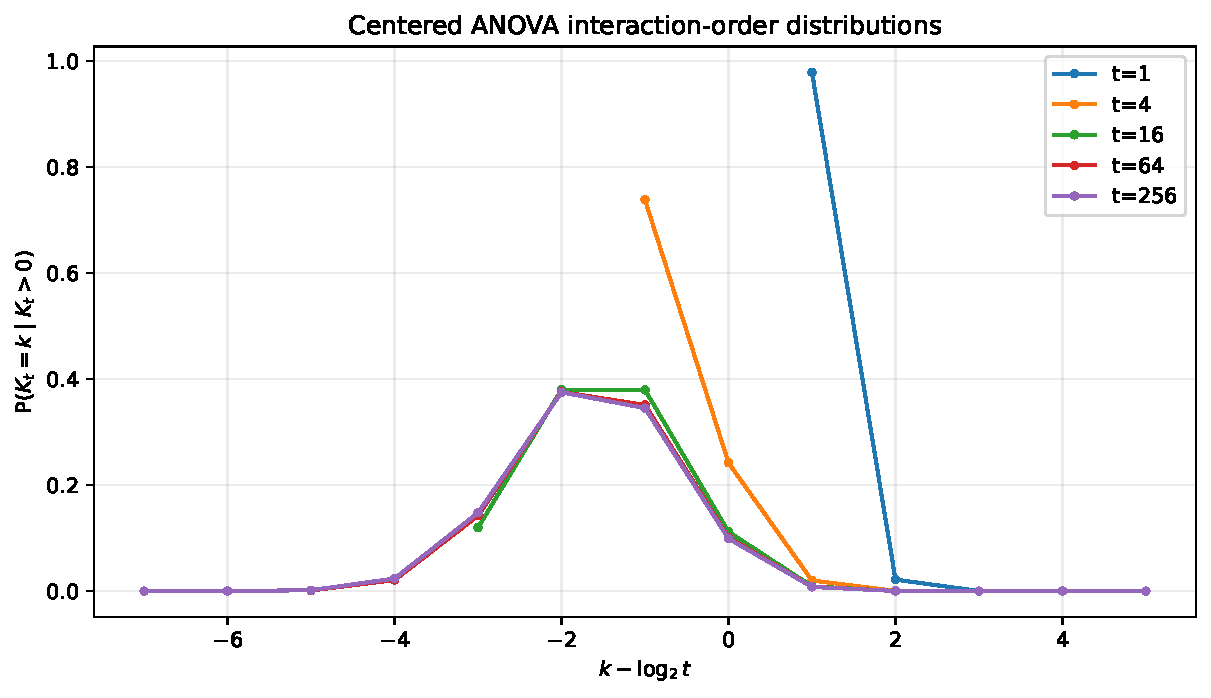
\includegraphics[width=0.88\textwidth]{figures/chaos_order_distributions.pdf}
\caption{Exact Poisson--binomial order weights
$\Prob(K_t=k\mid K_t>0)$ for several values of $t$.  As $t$ increases, the
interaction order translates roughly by $\log_2t$ rather than widening on a
central-limit scale.}
\label{fig:chaos-order}
\end{figure}

\subsection{Elementary local estimates}

\begin{lemma}[Activation bounds; \statusP]
\label{lem:p-bounds}
For $x\ge0$,
\begin{equation}
 0\le p(x)\le\min\left(1,\frac{x^2}{3}\right),
 \label{eq:p-bounds}
\end{equation}
For $x>0$ one also has
\begin{equation}
 0<1-p(x)=\frac{\tanh x}{x}\le\min\left(1,\frac1x\right),
 \qquad 1-p(0)=1.
 \label{eq:one-minus-p-bounds}
\end{equation}
Also
\begin{equation}
 p(x)=\frac{x^2}{3}-\frac{2x^4}{15}
      +\frac{17x^6}{315}-\frac{62x^8}{2835}+O(x^{10}).
 \label{eq:p-series}
\end{equation}
\end{lemma}

\begin{proof}
The lower bounds and $p<1$ follow from $0<\tanh x<x$ for $x>0$, with the
origin supplied by the continuous definitions in \eqref{eq:p-local}.
The inequality $\tanh x\ge x-x^3/3$ follows because the derivative of
$\tanh x-x+x^3/3$ is
$x^2-\tanh^2x\ge0$.  This proves $p(x)\le x^2/3$.  Since $\tanh x\le1$, the
second upper bound follows.  The series is obtained from the standard Taylor
series of $\tanh x/x$.
\end{proof}

\begin{corollary}[Sharp quadratic activation coefficient; \statusP]
\label{cor:sharp-activation-quadratic}
The coefficient $1/3$ in the global quadratic bound is optimal in the exact
local sense
\begin{equation}
 \boxed{
 \lim_{\substack{x\to0\\x\ne0}}\frac{p(x)}{x^2}=\frac13.}
 \label{eq:sharp-activation-quadratic}
\end{equation}
\end{corollary}

\begin{proof}
Apply l'Hopital's rule once to
$(x-\tanh x)/x^3$.  Its derivative quotient is
\[
 \frac{\tanh^2x}{3x^2}
 =\frac13\left(\frac{\tanh x}{x}\right)^2,
\]
which tends to $1/3$ because the totalized quotient $\tau$ is continuous and
$\tau(0)=1$.  For $x\ne0$, the original quotient equals $p(x)/x^2$.
\end{proof}

\begin{corollary}[Uniform interaction-count variance; \statusP]
\label{cor:K-variance-bound}
For all $t>0$,
\begin{equation}
 \Var(K_t)=\sum_{j\ge1}p(t2^{-j})\bigl(1-p(t2^{-j})\bigr)
 \le\frac{22}{9}.
 \label{eq:K-var-bound}
\end{equation}
\end{corollary}

\begin{proof}
For $0<t<1$, use $p(x)\le x^2/3$ to obtain
$\Var(K_t)\le\sum_jt^2/(3\cdot4^j)=t^2/9<1/9$.
For $t\ge1$, put $m=\lfloor\log_2t\rfloor$.  On $j\le m$ use
$p(1-p)\le1-p\le2^j/t$; hence the sum is less than $2$.  On $j>m$, use
$p(1-p)\le p\le t^2/(3\cdot4^j)$, whose tail is at most $4/9$.  The stated
uniform bound follows.
\end{proof}

\section{Marked tensor-Legendre chaos}
\label{sec:Legendre-chaos}

The one-dimensional Legendre expansion refines each active coordinate into a
local polynomial degree.  Let
\begin{equation}
 \ell_n(v)=\sqrt{2n+1}\,P_n(v),\qquad n\ge0,
 \label{eq:normalized-Legendre}
\end{equation}
so that $\{\ell_n\}_{n\ge0}$ is an orthonormal basis of
$L^2([-1,1],\dd v/2)$.  Define the modified spherical-Bessel coefficient
\begin{equation}
 i_n(x)=\frac12\int_{-1}^1\e^{xv}P_n(v)\dd v.
 \label{eq:i-n}
\end{equation}
Thus $i_0(x)=m(x)$ and the classical plane-wave/Legendre expansion reads
\begin{equation}
 \e^{xv}=\sum_{n\ge0}(2n+1)i_n(x)P_n(v)
        =\sum_{n\ge0}\sqrt{2n+1}\,i_n(x)\ell_n(v).
 \label{eq:local-Legendre-expansion}
\end{equation}

For a finitely supported multi-index
$\nu=(\nu_1,\nu_2,\ldots)\in\N_0^{(\N)}$, put
\begin{equation}
 \ell_\nu(V)=\prod_{j\ge1}\ell_{\nu_j}(V_j),
 \qquad \supp\nu=\{j:\nu_j>0\}.
 \label{eq:tensor-Legendre}
\end{equation}

\begin{proposition}[Local active-degree Parseval identity; \statusP]
\label{prop:local-Parseval}
For every real $x$,
\begin{equation}
 \boxed{
 \sum_{n\ge1}(2n+1)\frac{i_n(x)^2}{i_0(x)^2}
 =r(x).}
 \label{eq:local-Parseval}
\end{equation}
For $x\ne0$, define the local degree probabilities
\begin{equation}
 q_n(x)=\frac{(2n+1)i_n(x)^2}{m(2x)-m(x)^2},
 \qquad n\ge1.
 \label{eq:degree-mark}
\end{equation}
They sum to one and extend continuously to the origin by
\begin{equation}
 q_1(0)=1,
 \qquad q_n(0)=0\quad(n\ge2).
 \label{eq:degree-mark-zero}
\end{equation}
Consequently the local degree generating function has the unambiguous
continuous definition
\begin{equation}
 D(x,z)=
 \begin{cases}
  \displaystyle\sum_{n\ge1}q_n(x)z^n,&x\ne0,\\[0.4em]
  z,&x=0,
 \end{cases}
 \qquad |z|\le1.
 \label{eq:D-local}
\end{equation}
The convergence to $D(0,z)=z$ is uniform for $|z|\le1$.
\end{proposition}

\begin{proof}
Parseval applied to \eqref{eq:local-Legendre-expansion} gives
\[
 m(2x)=\frac12\int_{-1}^1\e^{2xv}\dd v
 =\sum_{n\ge0}(2n+1)i_n(x)^2.
\]
Subtract the $n=0$ term and divide by $m(x)^2$.  This proves
\eqref{eq:local-Parseval}; for $x\ne0$, the denominator in
\eqref{eq:degree-mark} is the same positive nonconstant local energy.  Finally,
$i_n(x)=x^n/(2n+1)!!+O(x^{n+2})$ and
$m(2x)-m(x)^2=x^2/3+O(x^4)$.  Hence $q_1(x)\to1$, while
$\sum_{n\ge2}q_n(x)=1-q_1(x)\to0$.  This proves
\eqref{eq:degree-mark-zero} and the asserted uniform convergence on the closed
unit disk.
\end{proof}

\begin{theorem}[Exact tensor-Legendre coefficients; \statusP]
\label{thm:tensor-Legendre}
The expansion
\begin{equation}
 \e^{tX}=\sum_{\nu\in\N_0^{(\N)}}c_\nu(t)\ell_\nu(V)
 \label{eq:tensor-expansion}
\end{equation}
converges in $L^2$, with
\begin{equation}
 \boxed{
 c_\nu(t)=M(t)
 \prod_{j\in\supp\nu}
 \frac{\sqrt{2\nu_j+1}\,i_{\nu_j}(x_j)}{i_0(x_j)}.}
 \label{eq:c-nu}
\end{equation}
For every finite $S$, summing the squared coefficients with support exactly
$S$ recovers the Hoeffding component:
\begin{equation}
 \sum_{\supp\nu=S}|c_\nu(t)|^2
 =\|H_S(t)\|_2^2.
 \label{eq:support-Legendre-energy}
\end{equation}
For $t\ne0$, the normalized \emph{nonconstant} squared tensor coefficients are
therefore generated by independent active indicators $B_j$ and, on active
coordinates, independent marks $N_j$ with
$\Prob(N_j=n\mid B_j=1)=q_n(x_j)$, conditioned on at least one activation.
At zero local field the continuous convention is $N_j=1$; it is harmless
because then $B_j=0$ almost surely.
\end{theorem}

\begin{proof}
Local Parseval is already established in \cref{prop:local-Parseval}.  Now fix
$N$ and use the exactly normalized conditional expectation
\[
 f_N=\E[\e^{tX}\mid\mathcal F_N]
 =M_{>N}(t)\prod_{j=1}^N\e^{x_jV_j}.
\]
Expanding these $N$ local factors by
\eqref{eq:local-Legendre-expansion} gives a finite tensor expansion in each
finite degree truncation; completeness and local Parseval give its $L^2$
limit.  Since
$M_{>N}(t)\prod_{j=1}^Ni_0(x_j)=M(t)$, its coefficient for every $\nu$ with
$\supp\nu\subset\{1,\ldots,N\}$ is exactly \eqref{eq:c-nu}.

The martingale $f_N$ converges in $L^2$ to $\e^{tX}$.  The nested finite tensor
bases therefore yield \eqref{eq:tensor-expansion} and show that the coefficient
squares sum to $\|\e^{tX}\|_2^2=M(2t)$.  A tensor coefficient lies in the
Hoeffding subspace indexed by $S$ exactly when $\supp\nu=S$; Parseval inside
that closed subspace proves \eqref{eq:support-Legendre-energy}.  Dividing the
local nonconstant energies by their sums gives the independent mark law, and
\cref{thm:active-set-law} supplies the independent active indicators.
\end{proof}

\begin{figure}[H]
\centering
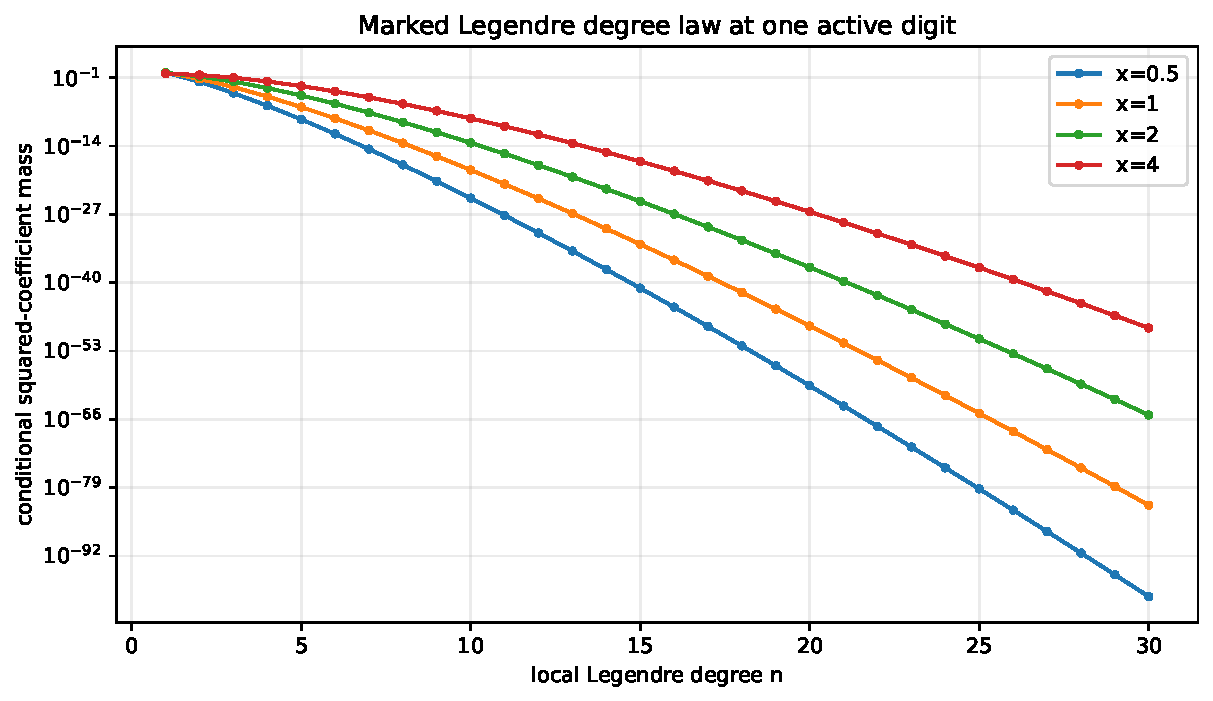
\includegraphics[width=0.84\textwidth]{figures/legendre_degree_marks.pdf}
\caption{The local degree mark in \eqref{eq:degree-mark}.  Larger local field
$x$ activates higher Legendre degrees, while the far dyadic tail remains
almost entirely degree one when it activates.}
\label{fig:degree-marks}
\end{figure}

\begin{corollary}[Joint interaction-degree generating function; \statusP]
\label{cor:joint-generating}
Let $u$ mark active-coordinate count and $z$ mark total Legendre degree.  The
normalized second-moment generating product, for $|u|,|z|\le1$, is
\begin{equation}
 \frac1{M(2t)}
 \sum_{\nu}|c_\nu(t)|^2u^{|\supp\nu|}z^{|\nu|_1}
 =\prod_{j\ge1}\left[(1-p_j)+p_ju\,D_j(z)\right],
 \label{eq:joint-degree-product}
\end{equation}
where $D_j(z)=D(x_j,z)$, so in particular $D_j(z)=z$ when $x_j=0$.
Equivalently, for $x_j\ne0$,
\begin{equation}
 D_j(z)=\sum_{n\ge1}
 \frac{(2n+1)i_n(x_j)^2}{m(2x_j)-m(x_j)^2}z^n.
 \label{eq:D-j}
\end{equation}
Conditioning away the all-zero multi-index gives the corresponding variance
law.
\end{corollary}

\begin{proof}
This is the probability-generating function of the independent marked process
identified by
\cref{thm:active-set-law,prop:local-Parseval,thm:tensor-Legendre}.
\end{proof}

\section{A sharp interaction bound for every smooth observable}
\label{sec:smooth-bound}

The exponential case is exactly factorized, but the dyadic geometry controls
much more general nonlinear observables.  Let $g\colon[-1,1]\to\R$ and
$f(V)=g(X)$, with $X$ as in \eqref{eq:X-centered}.  Write $g_S$ for the
Hoeffding component of $f$.

\subsection{A mixed-replacement identity}

For a finite set $S$, let $V'_j$ be independent copies of $V_j$, independent
of the original sequence.  If $h$ depends on $V_S$, define
\begin{equation}
 \Delta_Sh(V_S,V'_S)
 =\prod_{j\in S}\bigl(I-T'_j\bigr)h(V_S),
 \label{eq:mixed-difference}
\end{equation}
where $T'_j$ replaces $V_j$ by $V'_j$.

\begin{lemma}[Exact replacement norm; \statusP]
\label{lem:replacement-norm}
For every $h\in L^2(\sigma(V_j:j\in S))$,
\begin{equation}
 \E\bigl|\Delta_Sh(V_S,V'_S)\bigr|^2
 =2^{|S|}\left\|\prod_{j\in S}Q_jh\right\|_2^2.
 \label{eq:replacement-norm}
\end{equation}
\end{lemma}

\begin{proof}
For one coordinate,
\[
 \E|h(V)-h(V')|^2=2\E|h-\E h|^2=2\|Qh\|_2^2.
\]
Apply this identity successively to the coordinates in $S$.  At each step the
replacement difference commutes with all projections in the other
coordinates, and contributes a factor $2$ while applying the corresponding
$Q_j$.  Induction gives \eqref{eq:replacement-norm}.
\end{proof}

\begin{theorem}[Mixed-derivative interaction inequality; \statusP]
\label{thm:smooth-interaction}
Let $S\Subset\N$ with $|S|=k$, and suppose $g\in C^k([-1,1])$.  Then
\begin{equation}
 \boxed{
 \|g_S\|_2^2
 \le \frac{\|g^{(k)}\|_\infty^2}{3^k}
       \prod_{j\in S}a_j^2.}
 \label{eq:component-bound}
\end{equation}
Consequently, the total order-$k$ energy
\begin{equation}
 \Ecal_k(g)=\sum_{\substack{S\Subset\N\\|S|=k}}\|g_S\|_2^2
 \label{eq:E-k-general}
\end{equation}
satisfies
\begin{equation}
 \boxed{
 \Ecal_k(g)\le
 \frac{\|g^{(k)}\|_\infty^2}{3^k}
 e_k(a_1^2,a_2^2,\ldots),}
 \label{eq:order-bound-general}
\end{equation}
where $e_k$ is the $k$th elementary symmetric function.
\end{theorem}

\begin{proof}
Set
\[
 h_S(v_S)=\E\left[g(X)\mid V_S=v_S\right].
\]
Then $g_S=\prod_{j\in S}Q_jh_S$.  Differentiation under the expectation gives
\begin{equation}
 \frac{\partial^kh_S}{\prod_{j\in S}\partial v_j}(v_S)
 =\left(\prod_{j\in S}a_j\right)
 \E\left[g^{(k)}(X)\mid V_S=v_S\right].
 \label{eq:mixed-derivative-h}
\end{equation}
Repeated use of the fundamental theorem of calculus over the rectangle with
opposite corners $V_S$ and $V'_S$ yields
\[
 |\Delta_Sh_S|
 \le\|g^{(k)}\|_\infty
      \prod_{j\in S}a_j|V_j-V'_j|.
\]
By \cref{lem:replacement-norm},
\begin{align*}
 \|g_S\|_2^2
 &\le2^{-k}\|g^{(k)}\|_\infty^2
       \prod_{j\in S}a_j^2\E(V_j-V'_j)^2\\
 &=2^{-k}\|g^{(k)}\|_\infty^2
       \prod_{j\in S}a_j^2\left(\frac23\right)^k,
\end{align*}
which is \eqref{eq:component-bound}.  Summing over $|S|=k$ proves
\eqref{eq:order-bound-general}.
\end{proof}

\subsection{The exact dyadic and geometric-q factors}

The elementary symmetric function in \eqref{eq:order-bound-general} has a
closed $q$-Pochhammer form.

\begin{lemma}[Geometric elementary symmetric function; \statusI]
\label{lem:geometric-e}
For $0<Q<1$,
\begin{align}
 e_k(Q,Q^2,Q^3,\ldots)
 &=\frac{Q^{k(k+1)/2}}{(Q;Q)_k},
 \label{eq:e-start-one}\\
 e_k(1,Q,Q^2,\ldots)
 &=\frac{Q^{k(k-1)/2}}{(Q;Q)_k},
 \label{eq:e-start-zero}
\end{align}
where $(Q;Q)_k=\prod_{r=1}^k(1-Q^r)$.
\end{lemma}

\begin{proof}
The $q$-binomial theorem gives
\[
 \prod_{j\ge1}(1+zQ^j)
 =\sum_{k\ge0}\frac{Q^{k(k+1)/2}}{(Q;Q)_k}z^k.
\]
Coefficient comparison proves \eqref{eq:e-start-one}; adjoining the $j=0$
factor gives \eqref{eq:e-start-zero}.
\end{proof}

\begin{corollary}[Dyadic $q$-Pochhammer interaction bound; \statusP]
\label{cor:dyadic-interaction}
For the Fabius--Rvachev weights $a_j=2^{-j}$,
\begin{equation}
 \boxed{
 \Ecal_k(g)
 \le \frac{\|g^{(k)}\|_\infty^2}{3^k}
 \frac{4^{-k(k+1)/2}}{(1/4;1/4)_k}.}
 \label{eq:dyadic-interaction-bound}
\end{equation}
More generally, for
\begin{equation}
 X_q=(1-q)\sum_{j\ge0}q^jV_j,
 \qquad 0<q<1,
 \label{eq:X-q}
\end{equation}
whose coefficients sum to one,
\begin{equation}
 \boxed{
 \Ecal_{q,k}(g)
 \le\frac{\|g^{(k)}\|_\infty^2}{3^k}
 \frac{(1-q)^{2k}q^{k(k-1)}}{(q^2;q^2)_k}.}
 \label{eq:q-interaction-bound}
\end{equation}
\end{corollary}

\begin{proof}
Apply \cref{lem:geometric-e} with $Q=1/4$ in the dyadic case and with
$Q=q^2$ after factoring $(1-q)^{2k}$ in the geometric-$q$ case.
\end{proof}

\begin{remark}[What is sharp]
The constant $3^{-k}$ and the complete elementary-symmetric dependence on the
coordinate amplitudes cannot be reduced uniformly over all degree-$k$
polynomials: \cref{thm:monomial-sharp} below attains the bound at the highest
possible interaction order.  For a fixed nonpolynomial observable, the
inequality need not be equality because the mixed derivative varies across the
replacement rectangle.
\end{remark}

\subsection{Sharpness for monomials}

\begin{theorem}[Exact top-order monomial energy; \statusP]
\label{thm:monomial-sharp}
Let $g(x)=x^d$ with $d\ge1$.  Then $g_S=0$ whenever $|S|>d$.  If $|S|=d$, then
\begin{equation}
 g_S(V_S)=d!\prod_{j\in S}a_jV_j
 \label{eq:top-monomial-component}
\end{equation}
and
\begin{equation}
 \|g_S\|_2^2=\frac{(d!)^2}{3^d}\prod_{j\in S}a_j^2.
 \label{eq:top-monomial-norm}
\end{equation}
Consequently
\begin{equation}
 \boxed{
 \Ecal_d(x^d)=\frac{(d!)^2}{3^d}e_d(a_1^2,a_2^2,\ldots),}
 \label{eq:top-monomial-energy}
\end{equation}
so \eqref{eq:order-bound-general} is exact at $k=d$.
For the dyadic law,
\begin{equation}
 \Ecal_d(x^d)=
 \frac{(d!)^2}{3^d}
 \frac{4^{-d(d+1)/2}}{(1/4;1/4)_d}.
 \label{eq:dyadic-top-energy}
\end{equation}
\end{theorem}

\begin{proof}
Expand $X^d=(\sum_ja_jV_j)^d$.  A monomial in the coordinates involves at
most $d$ distinct indices, so no Hoeffding component of order above $d$ can
occur.  If $|S|=d$, the only term involving every coordinate in $S$ is the
multilinear term
$d!\prod_{j\in S}a_jV_j$; every other term either omits an index or has total
degree greater than $d$.  Since $\E V_j=0$, this multilinear term is already
pure in every coordinate.  Its squared norm is
$(d!)^2\prod_{j\in S}a_j^2\E V_j^2=(d!)^2 3^{-d}\prod a_j^2$.
Summing and using \cref{lem:geometric-e} proves the result.
\end{proof}

\begin{figure}[H]
\centering
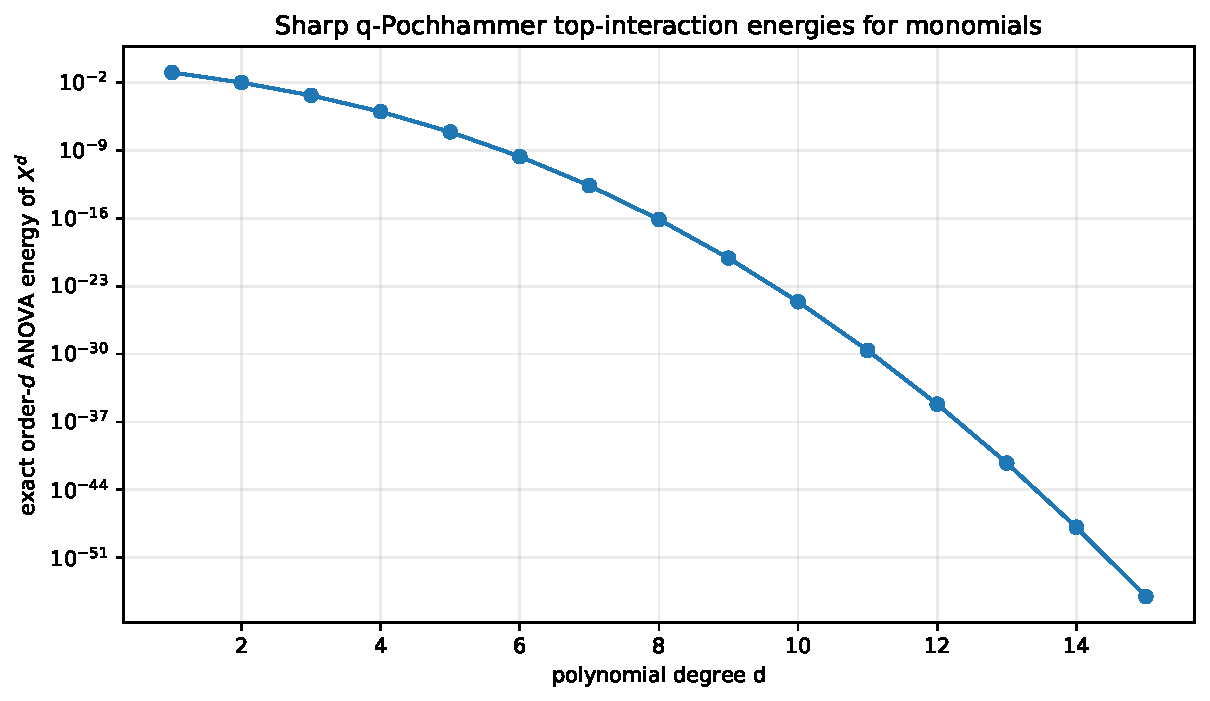
\includegraphics[width=0.82\textwidth]{figures/polynomial_top_energy.pdf}
\caption{The exact highest-order interaction energy
\eqref{eq:dyadic-top-energy}.  The quadratic exponent in the dyadic factor
forces superexponential decay even after multiplication by $(d!)^2$.}
\label{fig:polynomial-energy}
\end{figure}

\subsection{Exact polynomial components and Bell--Bernoulli tails}

For a finite $S$, write
\begin{equation}
 X_{S^c}=\sum_{j\notin S}a_jV_j,
 \qquad
 m_r^{(S^c)}=\E X_{S^c}^r,
 \qquad
 \mu_r=\E V_1^r=\frac{1+(-1)^r}{2(r+1)}.
 \label{eq:tail-moments}
\end{equation}

\begin{proposition}[All monomial Hoeffding components; \statusP]
\label{prop:all-monomial-components}
For $g(x)=x^d$ and a nonempty finite $S$,
\begin{equation}
 \boxed{
 g_S(V_S)=
 \sum_{\substack{\alpha_j\ge1\ (j\in S)\\|\alpha|\le d}}
 \frac{d!\,m_{d-|\alpha|}^{(S^c)}}
      {(d-|\alpha|)!\prod_{j\in S}\alpha_j!}
 \prod_{j\in S}a_j^{\alpha_j}
       \bigl(V_j^{\alpha_j}-\mu_{\alpha_j}\bigr).}
 \label{eq:all-monomial-components}
\end{equation}
The tail moments are complete Bell polynomials in the tail cumulants:
\begin{equation}
 m_r^{(S^c)}
 =\Bell_r\bigl(\kappa_1^{(S^c)},\ldots,\kappa_r^{(S^c)}\bigr),
 \qquad
 \kappa_r^{(S^c)}=\sum_{j\notin S}a_j^r\kappa_r(V_1).
 \label{eq:tail-Bell}
\end{equation}
For dyadic rational amplitudes, every coefficient in
\eqref{eq:all-monomial-components} is rational and can be generated exactly
from Bernoulli numbers.
\end{proposition}

\begin{proof}
Condition on $V_S$ and expand by the multinomial theorem:
\[
 \E[X^d\mid V_S]
 =\sum_{|\alpha|\le d}
 \frac{d!\,m_{d-|\alpha|}^{(S^c)}}
      {(d-|\alpha|)!\prod_{j\in S}\alpha_j!}
 \prod_{j\in S}(a_jV_j)^{\alpha_j}.
\]
Applying $Q_j$ annihilates every term with $\alpha_j=0$ and replaces
$V_j^{\alpha_j}$ by $V_j^{\alpha_j}-\mu_{\alpha_j}$ when
$\alpha_j\ge1$.  This proves \eqref{eq:all-monomial-components}.  Independence
makes cumulants additive and gives \eqref{eq:tail-Bell}.  The uniform cumulants
are rational Bernoulli combinations, and the dyadic amplitudes are rational.
\end{proof}

\begin{example}[The first two orders]
For $g(x)=x^2$,
\[
 g_{\{j\}}=a_j^2\left(V_j^2-\frac13\right),
 \qquad
 g_{\{i,j\}}=2a_ia_jV_iV_j.
\]
For $g(x)=x^3$,
\[
 g_{\{j\}}
 =a_j^3V_j^3+3a_jV_j\Var(X_{\{j\}^c}),
\]
while for distinct $i,j$,
\[
 g_{\{i,j\}}
 =3a_i^2a_j\left(V_i^2-\frac13\right)V_j
 +3a_ia_j^2V_i\left(V_j^2-\frac13\right),
\]
and $g_{\{i,j,k\}}=6a_ia_ja_kV_iV_jV_k$.
\end{example}

\subsection{Superexponential order truncation}

\begin{corollary}[Analytic-observable order tail; \statusP]
\label{cor:analytic-tail}
Suppose that for some $C,A>0$,
\begin{equation}
 \|g^{(k)}\|_\infty\le CA^kk!
 \qquad(k\ge0).
 \label{eq:analytic-derivative-bound}
\end{equation}
Then the dyadic order energies obey
\begin{equation}
 \Ecal_k(g)
 \le C^2\left(\frac{A^2}{3}\right)^k(k!)^2
 \frac{4^{-k(k+1)/2}}{(1/4;1/4)_k},
 \label{eq:analytic-order-bound}
\end{equation}
and the truncation after order $K$ satisfies
\begin{equation}
 \left\|g(X)-\sum_{|S|\le K}g_S\right\|_2^2
 \le\sum_{k>K}C^2\left(\frac{A^2}{3}\right)^k(k!)^2
 \frac{4^{-k(k+1)/2}}{(1/4;1/4)_k}.
 \label{eq:analytic-tail-bound}
\end{equation}
The right side decays faster than $\exp(-cK^2)$ for every fixed $A$.
\end{corollary}

\begin{proof}
Insert \eqref{eq:analytic-derivative-bound} into
\eqref{eq:dyadic-interaction-bound} and sum the orthogonal tail.  Since
$(1/4;1/4)_k$ decreases to the positive infinite product
$(1/4;1/4)_\infty$ and $\log(k!)=O(k\log k)$, the term
$4^{-k(k+1)/2}$ dominates by a negative quadratic exponent.
\end{proof}

\section{Small-field q-binomial asymptotics and Bell--Bernoulli structure}
\label{sec:q-small}

\subsection{Local expansion and the leading Gaussian-binomial row}

The local odds, totalized by $r(0)=0$, have the convergent expansion
\begin{equation}
 r(x)=\frac{x^2}{3}-\frac{x^4}{45}+\frac{2x^6}{945}
  -\frac{x^8}{4725}+O(x^{10}),
 \qquad |x|<\pi.
 \label{eq:r-series}
\end{equation}
For $x\ne0$ this is the Taylor expansion of $x\coth x-1$.
Let $Q=1/4$ and abbreviate
\begin{equation}
 E_k(Q)=\frac{Q^{k(k+1)/2}}{(Q;Q)_k}.
 \label{eq:E-k-Q}
\end{equation}

\begin{theorem}[Dyadic $q$-binomial chaos asymptotic; \statusP]
\label{thm:q-leading}
For every fixed $k\ge1$, as $t\to0$,
\begin{equation}
 \boxed{
 A_k(t)=\frac{t^{2k}}{3^k}
 \frac{4^{-k(k+1)/2}}{(1/4;1/4)_k}
 +O_k(t^{2k+2}).}
 \label{eq:A-leading}
\end{equation}
The first correction is
\begin{align}
 A_k(t)
 &=a^kt^{2k}E_k(Q)\\
 &\quad+ba^{k-1}t^{2k+2}
 \left(E_1(Q)E_k(Q)-(k+1)E_{k+1}(Q)\right)
 +O_k(t^{2k+4}),
 \label{eq:A-first-correction}
\end{align}
where $a=1/3$, $b=-1/45$, and $Q=1/4$.
\end{theorem}

\begin{proof}
Write $q_j=Q^j$.  From \eqref{eq:r-series},
\[
 r(t2^{-j})=at^2q_j+bt^4q_j^2+O(t^6q_j^3),
\]
uniformly in $j$ for $t$ in a fixed compact subinterval of $(-\pi,\pi)$.
The leading term of the elementary symmetric function $A_k$ is
$a^kt^{2k}e_k(q_1,q_2,\ldots)=a^kt^{2k}E_k(Q)$ by
\cref{lem:geometric-e}.

At relative order $t^2$, exactly one selected factor contributes its $b$ term.
The required symmetric sum is
\[
 T_k=\sum_jq_j^2e_{k-1}(q_1,\ldots,\widehat{q_j},\ldots).
\]
Multiplying $e_1e_k$ and separating whether the index from $e_1$ already
belongs to the $k$-set gives
\[
 e_1e_k=T_k+(k+1)e_{k+1}.
\]
This proves \eqref{eq:A-first-correction}; absolute geometric summability
controls the remainder.
\end{proof}

\begin{corollary}[General geometric-$q$ leading law; \statusP]
\label{cor:q-leading-general}
For $X_q$ in \eqref{eq:X-q}, let $A_{q,k}(t)$ be the order-$k$ coefficient for
$\e^{tX_q}$.  Then
\begin{equation}
 \boxed{
 A_{q,k}(t)
 \sim\left(\frac{(1-q)^2t^2}{3}\right)^k
 \frac{q^{k(k-1)}}{(q^2;q^2)_k}}
 \qquad(t\to0).
 \label{eq:general-q-leading}
\end{equation}
\end{corollary}

\begin{proof}
Use $r(x)\sim x^2/3$ and \eqref{eq:e-start-zero} with $Q=q^2$.
\end{proof}

\begin{figure}[H]
\centering
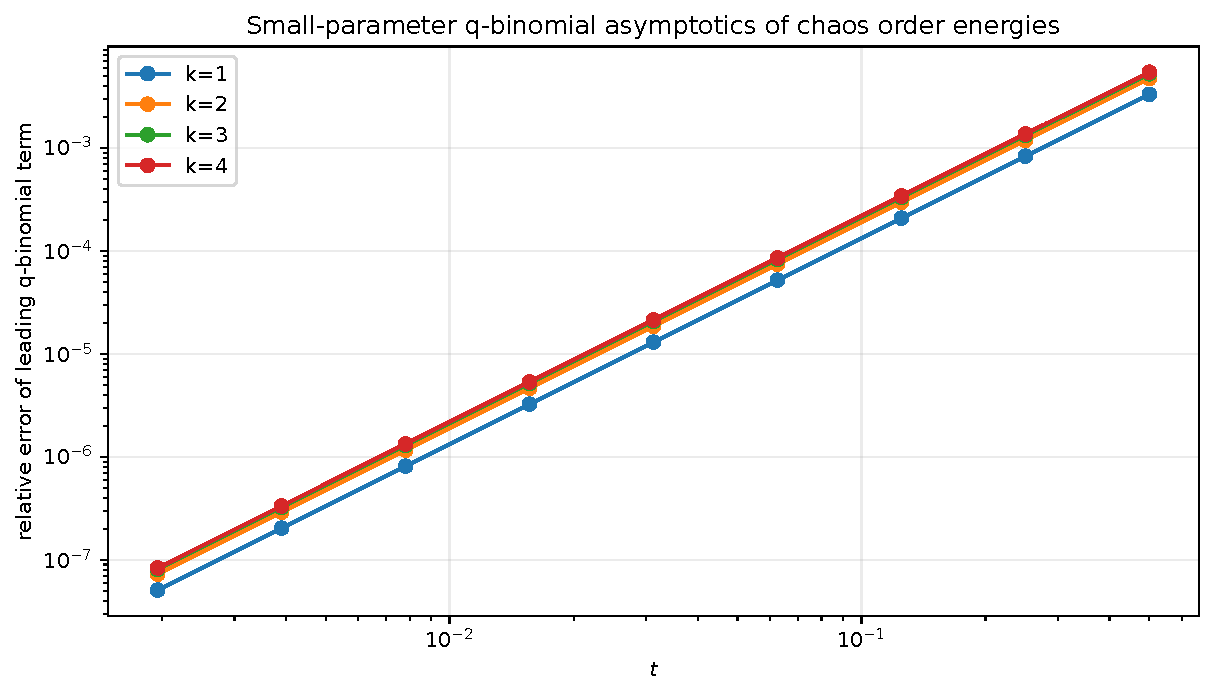
\includegraphics[width=0.84\textwidth]{figures/qbinomial_asymptotic_error.pdf}
\caption{Relative errors of the leading and first-corrected formulae for
$A_k(t)$.  The first correction in \eqref{eq:A-first-correction} improves the
power of $t$ by two, as predicted by the exact symmetric-sum calculation.}
\label{fig:q-error}
\end{figure}

\begin{corollary}[Small-field order law; \statusP]
\label{cor:small-order-law}
As $t\to0$,
\begin{equation}
 \Prob(K_t=k\mid K_t>0)
 \sim 3^{2-k}E_k(1/4)t^{2k-2},
 \qquad k\ge1.
 \label{eq:small-conditioned-order}
\end{equation}
In particular, the conditional variance energy concentrates at first order,
with the order-$k$ deficit carrying the exact Gaussian-binomial coefficient
$E_k(1/4)$.
\end{corollary}

\begin{proof}
Since $R-1=\sum_{k\ge1}A_k$ and
$A_1(t)\sim t^2E_1(1/4)/3=t^2/9$, divide \eqref{eq:A-leading} by this leading
term.
\end{proof}

\subsection{The total energy as a Bernoulli--Bell series}

The repository cumulants \eqref{eq:repo-cumulants} give an independent exact
expansion of the total normalized variance.

\begin{proposition}[Bell--Bernoulli energy coefficients; \statusP]
\label{prop:Bell-Bernoulli-energy}
Define
\begin{equation}
 \lambda_{2m}=(2^{2m}-2)\kappa_{2m}
 =\frac{(2^{2m}-2)2^{2m-1}B_{2m}}{m(4^m-1)},
 \quad m\ge1,
 \qquad
 \lambda_{2m+1}=0,\quad m\ge0.
 \label{eq:lambda-energy}
\end{equation}
Then, as Taylor series in the complex variable $t$,
\begin{align}
 \log R(t)
 &=\sum_{m\ge1}\lambda_{2m}\frac{t^{2m}}{(2m)!},
 \qquad |t|<\pi,
 \label{eq:logR-cumulants}\\
 R(t)
 &=\sum_{n\ge0}\Bell_n(\lambda_1,\ldots,\lambda_n)
                   \frac{t^n}{n!},
 \qquad |t|<4\pi,
 \label{eq:R-Bell}\\
 R(t)-1
 &=\sum_{m\ge1}\Bell_{2m}(0,\lambda_2,0,\lambda_4,\ldots)
                   \frac{t^{2m}}{(2m)!},
 \qquad |t|<4\pi.
 \label{eq:Rminus1-Bell}
\end{align}
Thus the sum over every nonempty interaction order is encoded by a complete
Bell transform of the Bernoulli--Mersenne cumulants.
\end{proposition}

\begin{proof}
The cumulant expansion of $\log M$ gives
\[
 \log R(t)=\log M(2t)-2\log M(t)
 =\sum_{n\ge1}(2^n-2)\kappa_n\frac{t^n}{n!}.
\]
Odd terms vanish.  Exponentiating by the complete Bell-polynomial formula
proves the result near the origin.  The displayed domains are the exact Taylor
disks.  Indeed $\log R$ first meets a zero of
$R(t)=m(t)/M(t)$ at $t=\pm\pi\ii$, whereas the apparent singularities of $R$
at $t=\pm2\pi\ii$ are removable: the simple zeros of $m(t)$ and $M(t)$
cancel.  At $t=\pm4\pi\ii$, $M(t)$ has two zero factors while $m(t)$ has only
one, so $R$ has a pole.  Thus the logarithmic series has radius $\pi$, while
the Taylor series for $R$ and $R-1$ have radius $4\pi$.
\end{proof}

\begin{remark}[Two Bell structures]
There are two distinct Bell transforms in the report.  Formula
\eqref{eq:A-Bell} reconstructs each \emph{interaction order} from power sums
of the local odds $r_j$.  Formula \eqref{eq:R-Bell} reconstructs the
\emph{sum over all orders} from cumulants of the one-dimensional Rvachev law.
Their equality after summing $A_k$ is a nontrivial bridge between local digit
sensitivity and global Bernoulli-number moment arithmetic.
\end{remark}

\section{Effective interaction dimension and a Mellin phase law}
\label{sec:effective-dimension}

The mean number of active coordinates is
\begin{equation}
 \mu(t)=\E K_t=\sum_{j\ge1}p(t2^{-j}).
 \label{eq:mu-def}
\end{equation}
It is distinct from $A_1(t)=\sum r_j$: the former counts the Bernoulli active
set underlying normalized coefficient energy, while the latter is the raw
first-order elementary symmetric sum.

\subsection{Refinement and convergent small-field series}

\begin{proposition}[Effective-dimension refinement; \statusP]
\label{prop:mu-refinement}
For $t\ge0$,
\begin{equation}
 \boxed{\mu(2t)-\mu(t)=p(t).}
 \label{eq:mu-refinement}
\end{equation}
If $|t|<\pi$, then
\begin{equation}
 \boxed{
 \mu(t)=\sum_{m\ge1}\frac{c_m}{4^m-1}t^{2m},
 \qquad
 c_m=-\frac{2^{2m+2}(2^{2m+2}-1)B_{2m+2}}{(2m+2)!}.}
 \label{eq:mu-small-series}
\end{equation}
For the geometric-$q$ law \eqref{eq:X-q},
\begin{align}
 \mu_q(t)&=\sum_{j\ge0}p((1-q)tq^j),
 \label{eq:mu-q-def}\\
 \mu_q(t)-\mu_q(qt)&=p((1-q)t),
 \label{eq:mu-q-refinement}\\
 \mu_q(t)&=\sum_{m\ge1}
 \frac{c_m(1-q)^{2m}}{1-q^{2m}}t^{2m},
 \qquad |(1-q)t|<\frac\pi2.
 \label{eq:mu-q-series}
\end{align}
\end{proposition}

\begin{proof}
The dyadic refinement is an index shift.  The Taylor series
$\tanh x/x=1-\sum_{m\ge1}c_mx^{2m}$, with the displayed Bernoulli
coefficients, converges for $|x|<\pi/2$.  In the dyadic sum the largest local
argument is $t/2$, so $|t|<\pi$ suffices.  Summing
$\sum_{j\ge1}4^{-mj}=1/(4^m-1)$ gives \eqref{eq:mu-small-series}.  The same
argument with coordinates $(1-q)q^j$ gives the geometric-$q$ identities.
\end{proof}

\begin{proposition}[Geometric activation dimension; \statusP]
\label{prop:geometric-activation-dimension}
Let $q,t\in\R$ with $|q|<1$, and define
\begin{equation}
 d_q(t)=\sum_{n\ge0}p\bigl(q^n(1-q)t\bigr).
 \label{eq:geometric-activation-dimension}
\end{equation}
The series is summable.  The resulting function is even and nonnegative,
vanishes at the origin, and satisfies
\begin{align}
 d_q(t)
 &=p\bigl((1-q)t\bigr)+d_q(qt),
 \label{eq:geometric-activation-refinement}\\
 d_q(t)-d_q(qt)
 &=p\bigl((1-q)t\bigr),
 \label{eq:geometric-activation-difference}\\
 d_q(t)&>0\iff t\ne0,
 \label{eq:geometric-activation-positive}\\
 d_q(t)
 &\le \frac{(1-q)t^2}{3(1+q)}.
 \label{eq:geometric-activation-quadratic}
\end{align}
At $q=0$ one has $d_0(t)=p(t)$.  More generally, for every integer $N\ge0$,
put
\[
 S_N(q,t)=\sum_{n=0}^{N-1}p\bigl(q^n(1-q)t\bigr).
\]
Then
\begin{align}
 d_q(t)&=S_N(q,t)+d_q(q^Nt),
 \label{eq:geometric-activation-prefix}\\
 S_N(q,t)&\le d_q(t)
 \le S_N(q,t)+
 \frac{(1-q)t^2}{3(1+q)}(q^2)^N.
 \label{eq:geometric-activation-enclosure}
\end{align}
At the dyadic value $q=1/2$, this is exactly the deterministic activation sum
\[
 d_{1/2}(t)=\sum_{n\ge0}p\bigl(2^{-(n+1)}t\bigr)
            =\sum_{j\ge1}p(t2^{-j}).
\]
Consequently, for every real $t$,
\begin{equation}
 d_{1/2}(2t)-d_{1/2}(t)=p(t),
 \qquad
 0\le d_{1/2}(t)\le\frac{t^2}{9},
 \qquad
 d_{1/2}(t)>0\iff t\ne0.
 \label{eq:formalized-dyadic-effective-dimension}
\end{equation}
\end{proposition}

\begin{proof}
The global estimate $p(x)\le x^2/3$ bounds the $n$-th term by
\[
 \frac{\bigl((1-q)t\bigr)^2}{3}(q^2)^n.
\]
Since $|q|<1$, comparison with the resulting geometric series proves
summability.  Factoring $1-q^2=(1-q)(1+q)$ gives the displayed quadratic
constant.  Removing the zeroth term gives the refinement, while removing the
first $N$ terms gives the exact prefix identity; applying the same quadratic
bound at $q^Nt$ yields the enclosure.  Positivity is already forced by the
zeroth term when $t\ne0$.  The dyadic statements are the specialization
$q=1/2$, with the index change $j=n+1$.
\end{proof}

The extension to $-1<q<0$ is an algebraic summability and refinement
statement.  The centered geometric-uniform probability law introduced in
\eqref{eq:X-q} still uses $0<q<1$.  Outside $|q|<1$, the Lean definition is a
totalized $\operatorname{tsum}$: no general summability or probability-law
claim is made there, although degenerate parameters may still give a
convergent series.  The report's separate identity
$\mu(t)=\E K_t=\sum_{j\ge1}p(t2^{-j})$ still depends on the active-count
construction; the proposition above proves only the deterministic activation
sum $d_{1/2}$.

\subsection{Mellin transform of the activation profile}

Define, initially in their convergence strips,
\begin{equation}
 \Mcal_p(s)=\int_0^\infty p(x)x^{s-1}\dd x,
 \qquad
 \Ical_p(s)=\int_0^\infty p'(x)x^s\dd x.
 \label{eq:Mellin-p-def}
\end{equation}

\begin{theorem}[Closed Mellin transforms; \statusP]
\label{thm:Mellin-p}
For $-2<\Re s<0$,
\begin{equation}
 \boxed{
 \Mcal_p(s)=
 2^{2-s}(1-2^{2-s})\Gamma(s-1)\zeta(s-1).}
 \label{eq:Mellin-p}
\end{equation}
Write $\Mcal_p^{\mathrm{cont}}$ for the meromorphic continuation supplied by
the right side of \eqref{eq:Mellin-p}.  For $-2<\Re s<1$,
\begin{equation}
 \boxed{
 \Ical_p(s)=-s\Mcal_p^{\mathrm{cont}}(s)
 =\frac{2^{2-s}(1-2^{2-s})\Gamma(s+1)\zeta(s-1)}{1-s}.}
 \label{eq:Mellin-pprime}
\end{equation}
The right sides are understood after filling removable singularities.
On $-2<\Re s<0$, $\Mcal_p^{\mathrm{cont}}$ agrees with the defining Mellin
integral $\Mcal_p$.  On the boundary line $\Re s=0$ and away from $s=0$, it
equals $-\Ical_p(s)/s$; the defining integral for $\Mcal_p$ is not absolutely
convergent there and does not have an ordinary improper limit.  By contrast,
the defining integral for $\Ical_p$ remains absolutely convergent on that
line.
\end{theorem}

\begin{proof}
By \cref{lem:p-bounds}, $p(x)=O(x^2)$ at zero and $p(x)=1+O(x^{-1})$ at
infinity, giving the strip $-2<\Re s<0$ for $\Mcal_p$.  Also
$p'(x)=O(x)$ at zero and $p'(x)=x^{-2}+O(\e^{-2x}/x)$ at infinity, giving
$-2<\Re s<1$ for $\Ical_p$.

Put
$J(s)=\int_0^\infty x^{s-1}\sech^2x\dd x$, which is holomorphic on the
half-plane $\Re s>0$.  The exponential expansion
\[
 \sech^2x=4\sum_{n\ge1}(-1)^{n-1}n\e^{-2nx}
\]
may be integrated term by term absolutely when $\Re s>2$, and there gives
\[
 J(s)=2^{2-s}\Gamma(s)(1-2^{2-s})\zeta(s-1).
\]
Both sides are holomorphic on $\Re s>0$ after filling their removable
singularities.  The identity theorem therefore extends this equality from
$\Re s>2$ to the whole half-plane $\Re s>0$; no conditionally justified
Fubini interchange is needed.

Now let $0<\Re s<1$.  Since
\[
 p'(x)=\frac{\tanh x-x\sech^2x}{x^2},
\]
integration by parts in the $\tanh x$ term is legitimate at both endpoints
and gives
\[
 \Ical_p(s)=\frac{s}{1-s}J(s).
\]
This proves \eqref{eq:Mellin-pprime} on $0<\Re s<1$, and analytic
continuation extends it to the full convergence strip of the left side.
Finally, integration by parts in \eqref{eq:Mellin-p-def} gives
$\Ical_p(s)=-s\Mcal_p(s)$ for $-2<\Re s<0$: the boundary term
$p(x)x^s$ vanishes because $p(x)=O(x^2)$ at zero and $p(x)=1+O(x^{-1})$ at
infinity.  The gamma recurrence
$\Gamma(s)=(s-1)\Gamma(s-1)$ gives \eqref{eq:Mellin-p}.
\end{proof}

\subsection{The logarithmically periodic mean}

For $\theta\in\R$, define the absolutely convergent renormalized sum
\begin{equation}
 P(\theta)=
 \sum_{k\le0}\left[p(2^{\theta-k})-1\right]
 +\sum_{k\ge1}p(2^{\theta-k}).
 \label{eq:P-theta}
\end{equation}
The estimates in \cref{lem:p-bounds} imply exponential convergence at both
ends.

\begin{theorem}[Exact dyadic phase expansion; \statusP]
\label{thm:mu-phase}
Let $t=2^{n+\theta}$ with $n\in\Z$, $0\le\theta<1$, and $t\ge1$.  Then
\begin{equation}
 \boxed{
 \mu(t)=n+P(\theta)+\varepsilon(t),
 \qquad 0\le\varepsilon(t)\le\frac2t.}
 \label{eq:mu-phase-exact}
\end{equation}
Moreover $P(\theta+1)=P(\theta)+1$.  Hence
\begin{equation}
 Q(\theta)=P(\theta)-\theta
 \label{eq:Q-def}
\end{equation}
is one-periodic and real analytic, and
\begin{equation}
 \boxed{
 \mu(t)=\log_2t+Q(\{\log_2t\})+O(t^{-1}).}
 \label{eq:mu-logperiodic}
\end{equation}
\end{theorem}

\begin{proof}
Reindex $j=n+k$ in \eqref{eq:mu-def}:
\[
 \mu(t)-n
 =\sum_{k=1-n}^0\left[p(2^{\theta-k})-1\right]
  +\sum_{k\ge1}p(2^{\theta-k}).
\]
Completing the first sum to $k=-\infty$ gives \eqref{eq:mu-phase-exact} with
\[
 \varepsilon(t)=\sum_{k\le-n}\left[1-p(2^{\theta-k})\right].
\]
Since $1-p(x)=\tanh x/x\le1/x$,
\[
 \varepsilon(t)\le\sum_{k\le-n}2^{k-\theta}=\frac2t.
\]
An index shift proves $P(\theta+1)=P(\theta)+1$.  Termwise differentiation is
permitted by exponential convergence of the differentiated tails; the Fourier
formula below gives real analyticity.
\end{proof}

Let $L=\log2$, $A$ be Glaisher's constant in the normalization
\begin{equation}
 \log A=\frac1{12}-\zeta'(-1),
 \label{eq:Glaisher}
\end{equation}
and set $\tau_n=2\pi n/L$.

\begin{theorem}[Fourier coefficients of the phase; \statusP]
\label{thm:Q-Fourier}
With the convention
\begin{equation}
 Q(\theta)=\sum_{n\in\Z}\widehat Q(n)\e^{2\pi\ii n\theta},
 \label{eq:Q-Fourier-series}
\end{equation}
one has
\begin{align}
 \boxed{
 \widehat Q(0)
 =\frac{11}{6}+\frac{\gamma-12\log A}{\log2},}
 \label{eq:Q0}\\
 \boxed{
 \widehat Q(n)
 =\frac{\Mcal_p^{\mathrm{cont}}(-\ii\tau_n)}{\log2}
 =\frac{\Ical_p(-\ii\tau_n)}{2\pi\ii n},
 \qquad n\ne0.}
 \label{eq:Qn}
\end{align}
In \eqref{eq:Qn}, the equal expression using $\Ical_p$ is an absolutely
convergent integral.
The coefficients decay exponentially; in particular the Fourier series and
all its termwise derivatives converge absolutely in a complex strip.
Numerically,
\begin{align}
 \widehat Q(0)&=-1.6404426943766166621038729\ldots,
 \label{eq:Q0-num}\\
 \widehat Q(1)&=
 (1.7087561142062823+1.3093920503208334\,\ii)10^{-6},
 \label{eq:Q1-num}\\
 2|\widehat Q(1)|&=4.3055104223684092\times10^{-6}.
 \label{eq:Q1-amplitude}
\end{align}
\end{theorem}

\begin{proof}
Differentiate \eqref{eq:P-theta} and unfold the logarithmic lattice.  For
$n\ne0$,
\begin{align*}
 \widehat{Q'}(n)
 &=\int_0^1L\sum_{k\in\Z}2^{\theta-k}
   p'(2^{\theta-k})\e^{-2\pi\ii n\theta}\dd\theta\\
 &=\int_{-\infty}^{\infty}\e^yp'(\e^y)
   \e^{-\ii\tau_ny}\dd y
 =\int_0^\infty p'(x)x^{-\ii\tau_n}\dd x
 =\Ical_p(-\ii\tau_n).
\end{align*}
Since $\widehat{Q'}(n)=2\pi\ii n\widehat Q(n)$, the nonzero formula follows
from \cref{thm:Mellin-p}.

For the mean, the Mellin transform of the harmonic sum is
\begin{equation}
 \int_0^\infty\mu(t)t^{s-1}\dd t
 =\frac{2^s}{1-2^s}\Mcal_p(s),
 \qquad -2<\Re s<0.
 \label{eq:Mellin-mu}
\end{equation}
At $s=0$,
\[
 \Mcal_p^{\mathrm{cont}}(s)=-\frac1s+c_0+O(s),
 \qquad
 c_0=\gamma-12\log A+\frac73\log2.
\]
Indeed, use
$\Gamma(s-1)=-s^{-1}+\gamma-1+O(s)$,
$\zeta(s-1)=-1/12+s\zeta'(-1)+O(s^2)$, and
$2^{2-s}(1-2^{2-s})=-12+28s\log2+O(s^2)$.
Also
\[
 \frac{2^s}{1-2^s}=-\frac1{s\log2}-\frac12+O(s).
\]
The double pole produces $\log_2t$, and its constant term is
$c_0/\log2-1/2$, which simplifies to \eqref{eq:Q0}.
Finally, Stirling's estimate for $\Gamma(-1-\ii\tau_n)$ in
\eqref{eq:Mellin-p} gives exponential decay in $|n|$.  The numerical values
were evaluated at 80 decimal digits by the accompanying program.
\end{proof}

\begin{figure}[H]
\centering
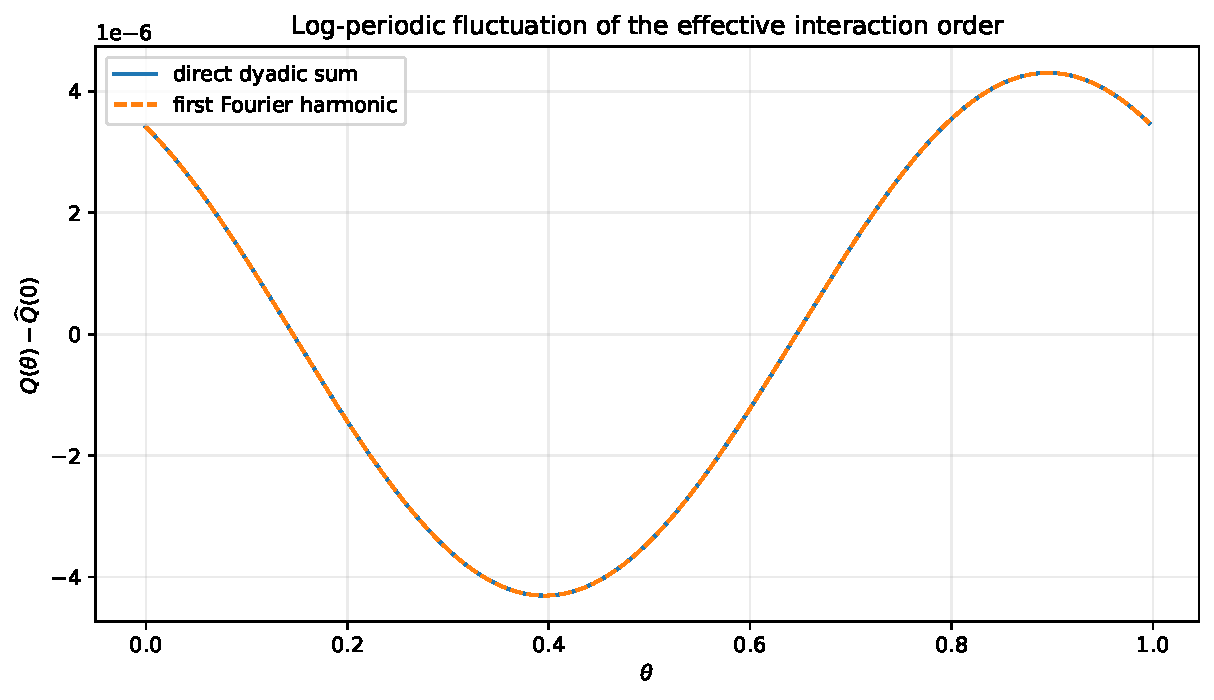
\includegraphics[width=0.88\textwidth]{figures/periodic_effective_dimension.pdf}
\caption{The periodic correction $Q(\theta)$.  The direct logarithmic-lattice
sum and the first Fourier harmonic are visually indistinguishable at this
scale; the total peak amplitude is only about $4.31\times10^{-6}$.}
\label{fig:periodic-Q}
\end{figure}

\subsection{A phase-indexed limiting distribution}

The bounded variance in \cref{cor:K-variance-bound} suggests that the active
count does not spread on a Gaussian scale.  The exact limit is a two-sided,
integer-valued phase law.

For $\theta\in[0,1)$, let
\begin{equation}
 p_{\theta,k}=p(2^{\theta-k}),\qquad k\in\Z,
 \label{eq:p-theta-k}
\end{equation}
and let $B_{\theta,k}$ be independent Bernoulli variables with these
parameters.  Define
\begin{equation}
 K_\theta=
 \sum_{k\le0}(B_{\theta,k}-1)+\sum_{k\ge1}B_{\theta,k}.
 \label{eq:K-theta}
\end{equation}
Both sums have only finitely many nonzero terms almost surely: the deficit
probabilities $1-p_{\theta,k}$ are summable on $k\le0$, and the activation
probabilities $p_{\theta,k}$ are summable on $k\ge1$.

\begin{theorem}[Dyadic phase law in total variation; \statusP]
\label{thm:phase-law}
Let $t=2^{n+\theta}$, $0\le\theta<1$, and $n\ge1$.  Then
\begin{equation}
 \boxed{
 \TV\bigl(K_t-n,K_\theta\bigr)\le\frac2t.}
 \label{eq:phase-TV}
\end{equation}
If $J_t$ denotes the variance-chaos order, that is,
\begin{equation}
 J_t\stackrel{\mathrm d}=K_t\mid(K_t>0),
 \label{eq:J-t}
\end{equation}
then
\begin{equation}
 \boxed{
 \TV\bigl(J_t-n,K_\theta\bigr)\le\frac4t.}
 \label{eq:conditioned-phase-TV}
\end{equation}
For every $z\in\C^\times$, the limiting bilateral probability generating
Laurent product is
\begin{equation}
 \boxed{
 \E z^{K_\theta}
 =\prod_{k\le0}\left[p_{\theta,k}+(1-p_{\theta,k})z^{-1}\right]
 \prod_{k\ge1}\left[(1-p_{\theta,k})+p_{\theta,k}z\right].}
 \label{eq:phase-pgf}
\end{equation}
Both products converge locally uniformly on $\C^\times$.
It has mean
\begin{equation}
 \E K_\theta=P(\theta).
 \label{eq:phase-mean}
\end{equation}
\end{theorem}

\begin{proof}
Use the same variables $B_{\theta,k}$ to couple the laws.  Reindexing the
original count gives
\[
 K_t=\sum_{k\ge1-n}B_{\theta,k}.
\]
Therefore
\[
 K_t-n
 =\sum_{k=1-n}^0(B_{\theta,k}-1)+\sum_{k\ge1}B_{\theta,k}.
\]
The coupled variables differ only if some omitted coarse index $k\le-n$ has a
deficit $B_{\theta,k}=0$.  By a union bound and
$1-p(x)\le1/x$,
\[
 \Prob(K_t-n\ne K_\theta)
 \le\sum_{k\le-n}(1-p_{\theta,k})
 \le\sum_{k\le-n}2^{k-\theta}=\frac2t.
\]
This proves \eqref{eq:phase-TV}.

Conditioning a law on an event of probability $1-\delta$ changes it by total
variation exactly $\delta$.  Here
\[
 \Prob(K_t=0)=\prod_{j\ge1}(1-p(t2^{-j}))
 \le1-p(t/2)=\frac{\tanh(t/2)}{t/2}\le\frac2t.
\]
The triangle inequality yields \eqref{eq:conditioned-phase-TV}.
The independent product \eqref{eq:phase-pgf} is immediate from
\eqref{eq:K-theta}.  On compact subsets of $\C^\times$, its coarse-factor
deviations are bounded by a constant times $1-p_{\theta,k}$ and its
fine-factor deviations by a constant times $p_{\theta,k}$; their sums converge.
This proves local uniform convergence.  Summing the expectations gives
precisely \eqref{eq:P-theta}.
\end{proof}

\begin{corollary}[No central-limit widening; \statusP]
\label{cor:no-CLT-width}
As $t\to\infty$, uniformly in the dyadic phase
$\{\log_2t\}\in[0,1)$,
\begin{equation}
 K_t=\log_2t+O_{\Prob}(1),
 \qquad
 J_t=\log_2t+O_{\Prob}(1).
 \label{eq:tight-order}
\end{equation}
Along each fixed phase $\theta$, every uniformly integrable family of powers
of $K_{2^{n+\theta}}-n$ has its moment converge to the corresponding moment of
$K_\theta$.  In particular,
\begin{equation}
 \Var(K_{2^{n+\theta}})\longrightarrow\Var(K_\theta).
 \label{eq:variance-phase-limit}
\end{equation}
More precisely, for $t=2^{n+\theta}$ with $n\ge1$,
\begin{equation}
 0\le \Var(K_\theta)-\Var(K_t)
 =\sum_{k\le-n}p_{\theta,k}(1-p_{\theta,k})
 \le\frac2t.
 \label{eq:variance-phase-tail}
\end{equation}
The family obeys the quasi-periodicity
\begin{equation}
 K_{\theta+1}\stackrel{\mathrm d}=K_\theta+1.
 \label{eq:phase-quasiperiodic}
\end{equation}
\end{corollary}

\begin{proof}
Tightness follows from \cref{thm:phase-law}, or directly from the uniformly
bounded variance and the bounded periodic mean correction, with $t\ge2$ (and
hence the stated $t\to\infty$ interpretation) understood.  Under the coupling
in \cref{thm:phase-law}, subtracting $n$ does not change variance and the only
terms missing from $K_t-n$ are the independent coarse deficits with $k\le-n$.
Consequently
\[
 \Var(K_\theta)-\Var(K_t)
 =\sum_{k\le-n}p_{\theta,k}(1-p_{\theta,k})
 \le\sum_{k\le-n}(1-p_{\theta,k})\le\frac2t,
\]
which proves \eqref{eq:variance-phase-tail} and
\eqref{eq:variance-phase-limit} directly, without inferring uniform
integrability of squares from bounded second moments.  Reindex
$B_{\theta+1,k}$ as $B_{\theta,k-1}$ in \eqref{eq:K-theta} to obtain
\eqref{eq:phase-quasiperiodic}.
\end{proof}

\begin{corollary}[Log-concavity and full support; \statusP]
\label{cor:phase-logconcave}
For every phase $\theta$, the mass function of $K_\theta$ is log-concave on
$\Z$ and strictly positive at every integer.  Its set of modes is therefore a
nonempty finite interval of consecutive integers.
\end{corollary}

\begin{proof}
Truncate \eqref{eq:K-theta} to $-N\le k\le N$.  Up to an integer shift, the
truncation is a finite Poisson--binomial sum, whose generating polynomial has
only real nonpositive zeros; Newton's inequalities imply log-concavity of its
coefficients.  The truncations converge in total variation, so the
coefficientwise inequalities pass to the limit.

For any prescribed integer, choose finitely many coarse deficits or fine
activations producing it.  That finite pattern has positive probability, and
the probability that no other tail event occurs is a positive convergent
product because the relevant tail probabilities are summable.  Hence the
support is all of $\Z$.  A log-concave sequence has a consecutive set of
maximizers; because this probability mass tends to zero in both tails, that
set is nonempty and finite.  Log-concavity alone does not bound its length by
two.
\end{proof}

\begin{figure}[H]
\centering
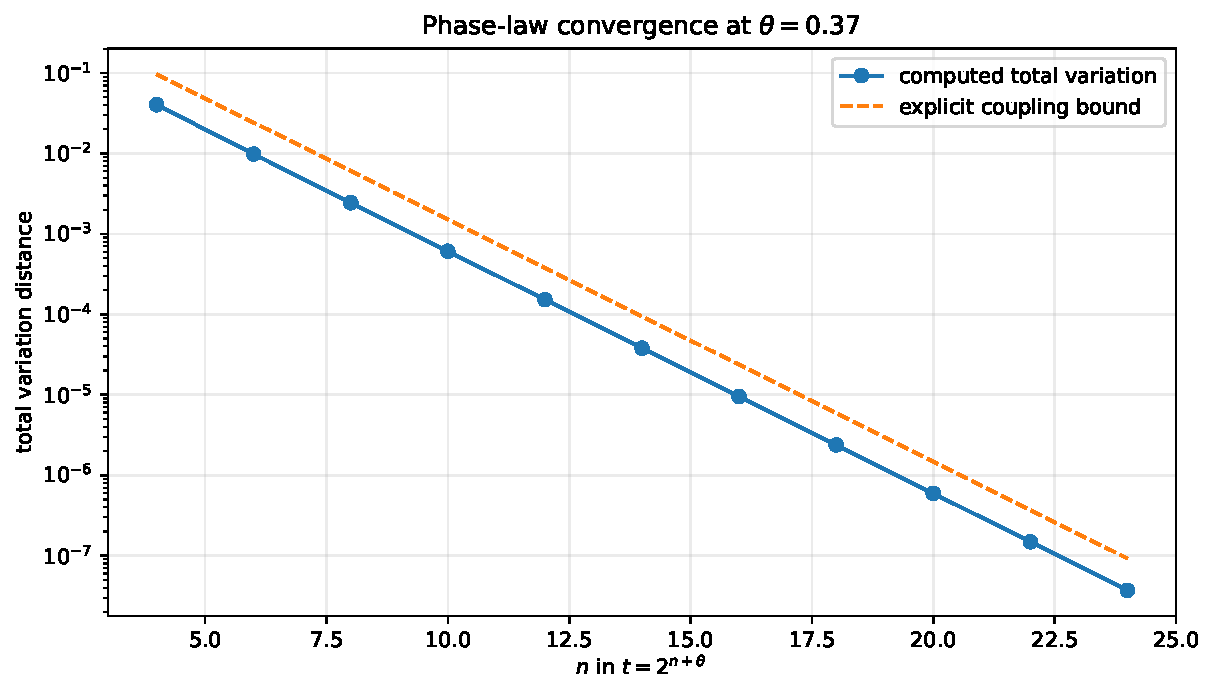
\includegraphics[width=0.86\textwidth]{figures/phase_limit_convergence.pdf}
\caption{Total-variation convergence at phase $\theta=0.37$.  The computed
error decays proportionally to $2^{-n}$ and remains below the explicit coupling
bound $2/t$.}
\label{fig:phase-TV}
\end{figure}

\section{The no-active atom and the negative Fabius Laplace endpoint}
\label{sec:Laplace-transfer}

Let
\begin{equation}
 L_F(s)=\E\e^{-sY}
 =\prod_{j\ge1}\frac{1-\e^{-s/2^j}}{s/2^j},
 \qquad s\ge0,
 \label{eq:Fabius-Laplace}
\end{equation}
be the negative Laplace transform of the Fabius random variable
\eqref{eq:Y-Fabius}.  The corpus studies
$\Lambda(s)=\log L_F(s)$ in detail, including an exact decomposition into a
quadratic logarithmic term, a log-periodic phase, and an exponentially small
remainder.

\begin{theorem}[Exact Laplace transfer of the ANOVA atom; \statusP]
\label{thm:Laplace-transfer}
For $t>0$,
\begin{equation}
 \boxed{
 \Prob(K_t=0)
 =\frac{2t}{1-\e^{-2t}}L_F(2t).}
 \label{eq:P0-Laplace}
\end{equation}
Equivalently,
\begin{equation}
 \boxed{
 \log\Prob(K_t=0)
 =\log(2t)-\log(1-\e^{-2t})+\Lambda(2t).}
 \label{eq:logP0-Laplace}
\end{equation}
Thus every exact or asymptotic statement for the repository's negative
Fabius Laplace product transfers immediately to the probability that the
exponential observable has no nonconstant active digit.
\end{theorem}

\begin{proof}
The Fabius law is symmetric: $Y\stackrel{\mathrm d}=1-Y$.  Therefore the
centered variable $X=2Y-1$ also satisfies
$X\stackrel{\mathrm d}=1-2Y$, and
\[
 M(t)=\E\e^{tX}=\e^t\E\e^{-2tY}=\e^tL_F(2t).
\]
Now use \eqref{eq:P0} and
$m(t)=\sinh t/t=(\e^t-\e^{-t})/(2t)$.
\end{proof}

\begin{corollary}[Transported quadratic-log phase; \statusP+\statusI]
\label{cor:transported-phase}
Suppose the repository decomposition is written in the normalization
\begin{equation}
 \Lambda(s)=
 -\frac{(\log s)^2}{2\log2}+\frac12\log s
 +\Psi(\log_2s)+E(s),
 \label{eq:repo-Lambda-form}
\end{equation}
where $\Psi$ is one-periodic and $E(s)$ is the explicit exponentially small
remainder supplied there.  Then
\begin{align}
 \log\Prob(K_t=0)
 &=-\frac{(\log(2t))^2}{2\log2}
   +\frac32\log(2t)
   +\Psi(1+\log_2t)\\
 &\quad-\log(1-\e^{-2t})+E(2t).
 \label{eq:P0-transported-asymptotic}
\end{align}
In particular, the same log-periodic endpoint phase controls a concrete
high-dimensional sensitivity event.
\end{corollary}

\begin{proof}
Substitute $s=2t$ from \eqref{eq:repo-Lambda-form} into
\eqref{eq:logP0-Laplace}.  Periodicity permits replacing
$\Psi(1+\log_2t)$ by $\Psi(\log_2t)$ if desired.
\end{proof}

\begin{remark}[Distinct periodic functions]
The periodic correction $Q$ in \cref{thm:Q-Fourier} concerns the \emph{mean
number} of active digits and has Fourier coefficients governed by the Mellin
transform of $p$.  The imported phase $\Psi$ in
\eqref{eq:repo-Lambda-form} concerns the \emph{probability of zero} active
digits and comes from the Fabius Laplace product.  They arise from the same
dyadic lattice but are not the same function.
\end{remark}

\section{Thue--Morse corners inside the continuous digit chaos}
\label{sec:Thue-Morse}

The original coordinates are uniform rather than binary.  Nevertheless each
uniform variable admits the independent sign--magnitude factorization
\begin{equation}
 V_j=R_jU_j,
 \qquad R_j\in\{-1,1\}\text{ Rademacher},
 \qquad U_j\sim\operatorname{Unif}[0,1].
 \label{eq:sign-magnitude}
\end{equation}
This refines the continuous chaos into Walsh sign interactions and magnitude
interactions.

For $a\in\R$, let
\begin{equation}
 \Delta_a g(x)=g(x+a)-g(x-a).
 \label{eq:symmetric-difference}
\end{equation}

\begin{theorem}[Continuous Thue--Morse corner identity; \statusP]
\label{thm:TM-corner}
Let $a_1,\ldots,a_N>0$, let $I\subset\R$ be an open interval containing
\[
 \left[x-\sum_{j=1}^Na_j,\ x+\sum_{j=1}^Na_j\right],
\]
and suppose $g\in C^N(I)$.  Then
\begin{align}
 \Delta_{a_1}\cdots\Delta_{a_N}g(x)
 &=\sum_{\varepsilon\in\{-1,1\}^N}
   \left(\prod_{j=1}^N\varepsilon_j\right)
   g\left(x+\sum_{j=1}^Na_j\varepsilon_j\right)
 \label{eq:corner-sign-sum}\\
 &=\int_{-a_1}^{a_1}\cdots\int_{-a_N}^{a_N}
   g^{(N)}(x+u_1+\cdots+u_N)\dd u_1\cdots\dd u_N.
 \label{eq:corner-integral}
\end{align}
For the dyadic amplitudes $a_j=2^{-j}$,
\begin{equation}
 \boxed{
 \Delta_{2^{-1}}\cdots\Delta_{2^{-N}}g(x)
 =(-1)^N\sum_{k=0}^{2^N-1}(-1)^{s_2(k)}
 g\left(x-(1-2^{-N})+\frac{k}{2^{N-1}}\right),}
 \label{eq:TM-corner}
\end{equation}
where $s_2(k)$ is the binary digit sum.  Hence the corner annihilates every
polynomial of degree below $N$, while
\begin{equation}
 \Delta_{2^{-1}}\cdots\Delta_{2^{-N}}x^N
 =N!\,2^{-N(N-1)/2}.
 \label{eq:TM-top}
\end{equation}
\end{theorem}

\begin{proof}
Expanding the product of symmetric differences gives
\eqref{eq:corner-sign-sum}.  The one-dimensional identity
$g(x+a)-g(x-a)=\int_{-a}^ag'(x+u)\dd u$, iterated $N$ times, gives
\eqref{eq:corner-integral}.

For dyadic amplitudes, write
$\varepsilon_j=2b_j-1$ and
$k=\sum_{j=1}^Nb_j2^{N-j}$.  Then
\[
 \sum_{j=1}^N2^{-j}\varepsilon_j
 =-(1-2^{-N})+\frac{k}{2^{N-1}},
 \qquad
 \prod_{j=1}^N\varepsilon_j=(-1)^N(-1)^{s_2(k)}.
\]
This proves \eqref{eq:TM-corner}.  If $\deg g<N$, then $g^{(N)}=0$ in
\eqref{eq:corner-integral}.  For $g(x)=x^N$, the integrand is $N!$ and the
box volume is
$\prod_j2a_j=2^N2^{-N(N+1)/2}=2^{-N(N-1)/2}$.
\end{proof}

\begin{corollary}[Highest Walsh sign coefficient; \statusP]
\label{cor:Walsh-corner}
Condition on the magnitudes $U_1,\ldots,U_N$ and on a tail variable $Z$
independent of the signs.  Then
\begin{equation}
 \E_R\left[
 g\left(Z+\sum_{j=1}^Na_jR_jU_j\right)
 \prod_{j=1}^NR_j\right]
 =2^{-N}\Delta_{a_1U_1}\cdots\Delta_{a_NU_N}g(Z).
 \label{eq:Walsh-corner}
\end{equation}
At $U_1=\cdots=U_N=1$ and $a_j=2^{-j}$, the highest sign interaction is the
canonical Thue--Morse/Prouhet corner \eqref{eq:TM-corner}.
\end{corollary}

\begin{proof}
The conditional expectation over $2^N$ equally likely sign vectors is
$2^{-N}$ times \eqref{eq:corner-sign-sum} with amplitudes $a_jU_j$.
\end{proof}

\begin{remark}
The corner identity explains why Thue--Morse cancellation and high-order
functional ANOVA meet naturally but are not identical.  Hoeffding projection
centers the full uniform coordinate; Walsh projection centers only its sign
conditional on its magnitude.  The sign--magnitude refinement provides the
precise bridge.
\end{remark}

\section[Lambert-W cutoffs for Legendre chaos]
{Lambert-W degree cutoffs for Legendre chaos}
\label{sec:Lambert-cutoff}

The corpus uses Lambert $W$ primarily in endpoint inversion.  Polynomial chaos
creates a different occurrence: inversion of factorial Legendre-coefficient
decay.

\begin{proposition}[Rodrigues bound for local coefficients; \statusP]
\label{prop:Rodrigues-bound}
For $n\ge0$ and $x\in\C$,
\begin{equation}
 i_n(x)=\frac{x^n}{2^{n+1}n!}
 \int_{-1}^1\e^{xv}(1-v^2)^n\dd v,
 \label{eq:i-Rodrigues}
\end{equation}
and hence
\begin{equation}
 \boxed{
 |i_n(x)|\le\e^{|x|}\frac{|x|^n}{(2n+1)!!}.}
 \label{eq:i-bound}
\end{equation}
\end{proposition}

\begin{proof}
Insert Rodrigues' formula
$P_n(v)=(2^nn!)^{-1}\frac{\dd^n}{\dd v^n}(v^2-1)^n$ into
\eqref{eq:i-n}.  Integrating by parts $n$ times produces
\eqref{eq:i-Rodrigues}; all boundary terms vanish because $(1-v^2)^n$ has the
required endpoint zeros.  Next,
\[
 \int_{-1}^1(1-v^2)^n\dd v
 =\frac{2^{2n+1}(n!)^2}{(2n+1)!}.
\]
Using $(2n+1)!!=(2n+1)!/(2^nn!)$ gives \eqref{eq:i-bound}.
\end{proof}

\begin{corollary}[Lambert-$W$ inversion rule; \statusP]
\label{cor:Lambert-degree}
Fix $x\ne0$ and define the exact envelope and its monotone-tail threshold by
\begin{equation}
 b_n(x)=\e^{|x|}\frac{|x|^n}{(2n+1)!!},
 \qquad
 N_x=\left\lceil\frac{|x|}{2}\right\rceil.
 \label{eq:degree-envelope}
\end{equation}
For every $\varepsilon>0$, define
\begin{equation}
 n_\varepsilon(x)=
 \min\left\{n\in\N_0:n\ge N_x\ \text{and}\ b_n(x)\le\varepsilon\right\}.
 \label{eq:n-epsilon-def}
\end{equation}
This set is nonempty, and the resulting cutoff is certified for the entire
tail:
\begin{equation}
 |i_m(x)|\le b_m(x)\le\varepsilon
 \qquad\text{for every }m\ge n_\varepsilon(x).
 \label{eq:degree-certified-tail}
\end{equation}
As $\varepsilon\downarrow0$, define
\begin{equation}
 A_\varepsilon=\log\frac{\e^{|x|}}{\varepsilon}.
 \label{eq:A-epsilon}
\end{equation}
The degree at which the envelope \eqref{eq:i-bound} reaches tolerance
$\varepsilon$ has the leading inversion
\begin{equation}
 \boxed{
 n_\varepsilon(x)
 \sim\frac{A_\varepsilon}
 {W_0\!\left(\dfrac{2A_\varepsilon}{\e|x|}\right)}.}
 \label{eq:Lambert-degree}
\end{equation}
Thus \eqref{eq:Lambert-degree} is an asymptotic initial guess for the exact,
tail-valid cutoff \eqref{eq:n-epsilon-def}, not merely for a single coefficient.
\end{corollary}

\begin{proof}
The exact ratio
\[
 \frac{b_{n+1}(x)}{b_n(x)}=\frac{|x|}{2n+3}<1
 \qquad(n\ge N_x)
\]
shows that the envelope is decreasing there and tends to zero, so the defining
set is nonempty and its minimum certifies every later envelope value.  This
proves \eqref{eq:degree-certified-tail} from
\cref{prop:Rodrigues-bound}.

For the asymptotic, put
\[
 F_x(n)=\log\bigl((2n+1)!!\bigr)-n\log|x|,
\]
so that $b_n(x)\le\varepsilon$ is equivalent to
$F_x(n)\ge A_\varepsilon$.  As $\varepsilon\downarrow0$ one has
$n_\varepsilon(x)\to\infty$.  Hence, for all sufficiently small
$\varepsilon$, minimality on the monotone tail gives, with
$n=n_\varepsilon(x)$,
\[
 F_x(n-1)<A_\varepsilon\le F_x(n).
\]
Since
\[
 F_x(n)-F_x(n-1)=\log\frac{2n+1}{|x|}=O(\log n),
\]
this sandwiches the threshold sharply enough to give
$F_x(n)=A_\varepsilon+O(\log n)$.  Stirling's formula gives
\[
 \log\bigl((2n+1)!!\bigr)
 =n\log\frac{2n}{\e}+O(\log n).
\]
Therefore the exact minimal cutoff satisfies
\[
 n\log\frac{2n}{\e|x|}=A_\varepsilon+O(\log n).
\]
Solving the leading equation with $W_0(z)\e^{W_0(z)}=z$ yields
\eqref{eq:Lambert-degree}.  Moreover, the derivative of
$y\mapsto y\log(2y/(\e|x|))$ is
$1+\log(2y/(\e|x|))\to\infty$.  Hence the $O(\log n)$ perturbation moves the
inverse by $o(n)$ and does not affect the asymptotic ratio.
\end{proof}

\begin{remark}[Adaptive tensor truncation]
At digit $j$, the local field is $x_j=t2^{-j}$.  Formula
\eqref{eq:Lambert-degree} therefore assigns a different degree cutoff to every
active digit.  Coarse digits may require several Legendre modes, while far-tail
digits have $|x_j|\ll1$ and their conditional mark law is overwhelmingly
concentrated at degree one.  This is substantially more efficient than a
rectangular tensor-degree cutoff.
\end{remark}

\section{Reproducible exact and numerical experiments}
\label{sec:numerics}

The archive contains \path{experiments.py}, a self-contained deterministic
program using high-precision arithmetic and standard special-function
routines.  It does not use Monte Carlo simulation.  Its role is to check
transcriptions, illustrate limiting laws, and quantify approximation errors;
none of the analytic theorems depends on a floating-point experiment.

\subsection{Certified truncation policy}

Every countable probability sum uses the global inequality
$p(x)\le x^2/3$.  If the sum is truncated after digit $J$, then
\begin{equation}
 \sum_{j>J}p(t2^{-j})
 \le\frac{t^2}{3}\sum_{j>J}4^{-j}
 =\frac{t^2}{9\,4^J}.
 \label{eq:numerical-tail-bound}
\end{equation}

\begin{corollary}[Certified dyadic activation truncation; \statusP]
\label{cor:dyadic-activation-truncation}
For every $t\in\R$ and integer $N\ge0$,
\begin{equation}
 d_{1/2}(t)
 =\sum_{n=0}^{N-1}p\bigl(2^{-(n+1)}t\bigr)
 +d_{1/2}(2^{-N}t).
 \label{eq:dyadic-activation-prefix}
\end{equation}
The omitted tail is nonnegative and has the certified bound
\begin{equation}
 0\le d_{1/2}(2^{-N}t)
 \le\frac{t^2}{9\,4^N}.
 \label{eq:dyadic-activation-tail}
\end{equation}
Equivalently, after retaining the report coordinates $j=1,\ldots,N$,
\[
 0\le\sum_{j>N}p(t2^{-j})
 \le\frac{t^2}{9\,4^N}.
\]
\end{corollary}

\begin{proof}
The prefix identity is \eqref{eq:geometric-activation-prefix} at $q=1/2$.
Nonnegativity follows termwise, and the quadratic estimate applied at
$2^{-N}t$ gives
\[
 d_{1/2}(2^{-N}t)\le\frac{(2^{-N}t)^2}{9}
 =\frac{t^2}{9\,4^N}.
\]
\end{proof}

The same bound controls the probability that any omitted Bernoulli activation
occurs.  Hyperbolic-product tails use the analogous estimate
$0\le\log m(x)\le x^2/6$ for real $x$.  The chosen precision is 80 decimal
digits; CSV files record every truncation depth and bound.

\subsection{What the program verifies}

The driver performs the following independent computations:
\begin{enumerate}
\item direct logarithmic-lattice evaluation of $Q(\theta)$ and comparison with
      its Mellin Fourier series;
\item exact Poisson--binomial convolutions for the conditioned chaos-order law;
\item total-variation convergence to a deep finite approximation of the phase
      law and comparison with the bound $2/t$;
\item elementary-symmetric computation of $A_k(t)$ and comparison with
      \eqref{eq:A-leading} and \eqref{eq:A-first-correction};
\item local Legendre Parseval checks using modified spherical Bessel functions;
\item exact rational evaluation of the monomial top energy
      \eqref{eq:dyadic-top-energy};
\item independent comparison of the product formula for $\Prob(K_t=0)$ with
      the negative Fabius Laplace product \eqref{eq:P0-Laplace}.
\end{enumerate}

\begin{table}[H]
\centering
\caption{Selected reproducibility checks from
\texttt{data/numerical\_summary.txt}.}
\label{tab:numerical-summary}
\begin{tabularx}{0.96\textwidth}{@{}l>{\raggedleft\arraybackslash}X@{}}
\toprule
Quantity & Computed value \\
\midrule
$\widehat Q(0)$
& $-1.6404426943766166621038729159$ \\
$2|\widehat Q(1)|$
& $4.30551042236840917\times10^{-6}$ \\
Maximum direct/Fourier error for $Q$ on the plotted grid
& $5.8207661\times10^{-11}$ \\
Maximum independent error in \eqref{eq:P0-Laplace}
& $9.2975205\times10^{-26}$ \\
Maximum degree-64 local Parseval error
& $6.2172489\times10^{-15}$ \\
Maximum relative error of the first-corrected $A_k$ grid
& $3.2116589\times10^{-5}$ \\
Phase TV error at $(\theta,n)=(0.37,24)$
& $3.7100290\times10^{-8}$ \\
Theoretical coupling bound at the same point
& $9.2332142\times10^{-8}$ \\
Exact top energy $\Ecal_{10}(x^{10})$
& $2.4950901155034477\times10^{-25}$ \\
\bottomrule
\end{tabularx}
\end{table}

\begin{table}[H]
\centering
\caption{The no-active atom from two independent products.}
\label{tab:no-active}
\begin{tabular}{@{}rrrr@{}}
\toprule
$t$ & $\Prob(K_t=0)$ & $\log\Prob(K_t=0)$ & absolute discrepancy \\
\midrule
$1$   & $8.99201007738952\times10^{-1}$ & $-0.1062486791$ & $9.30\times10^{-26}$ \\
$8$   & $8.24685731480165\times10^{-2}$ & $-2.4953379898$ & $8.53\times10^{-27}$ \\
$32$  & $6.44285582709265\times10^{-4}$ & $-7.3473684787$ & $6.66\times10^{-29}$ \\
$128$ & $3.14592569682258\times10^{-7}$ & $-14.9719874649$ & $3.25\times10^{-32}$ \\
$256$ & $2.45775445064264\times10^{-9}$ & $-19.8240177288$ & $2.54\times10^{-34}$ \\
\bottomrule
\end{tabular}
\end{table}

\subsection{Reproduction command}

From the archive root, run
\begin{center}
\setlength{\fboxsep}{7pt}
\fbox{\texttt{python experiments.py --root .}}
\end{center}
This regenerates all CSV files, the numerical summary, and both vector and
raster versions of the figures.  Dependencies and tested minimum versions are
listed in \path{requirements.txt}.

\begin{warning}
The Fourier comparison error in \cref{tab:numerical-summary} is dominated by
the deliberately finite direct-lattice evaluation, not by the four-harmonic
Fourier series: the second Fourier harmonic is already of order $10^{-12}$ and
subsequent harmonics are dramatically smaller.  Likewise, finite
Poisson--binomial calculations are evidence for, not substitutes for, the
coupling proof in \cref{thm:phase-law}.
\end{warning}

\section{Conjectures and frontier research program}
\label{sec:frontiers}

The proved structure opens several questions that do not reduce to the
repository's existing endpoint, spectral, or $q$-inverse programs.

\subsection{Mode locking in the phase law}

\begin{conjecture}[Unique phase mode]
\label{conj:unique-mode}
For every $\theta\in[0,1)$, the full-support log-concave law $K_\theta$ has a
unique mode except at finitely many phases.  At each exceptional phase exactly
two adjacent integers tie, and every crossing is transversal.
\end{conjecture}

Log-concavity from \cref{cor:phase-logconcave} reduces this to control of
adjacent probability ratios.  The quasi-periodicity
$K_{\theta+1}\stackrel{\mathrm d}=K_\theta+1$ suggests one mode transition per
period, but the extremely small oscillation of the mean does not by itself
prove that picture.  A promising route is to differentiate the Laurent
product \eqref{eq:phase-pgf} and establish strict monotonicity of the relevant
coefficient ratio.

\subsection{Differential algebra of the chaos products}

\begin{conjecture}[Differential transcendence]
\label{conj:differential-transcendence}
For generic algebraic $z\ne0,1$, neither $t\mapsto\Ccal(t,z)$ nor
$t\mapsto\sum_{j\ge1}p(t2^{-j})$ satisfies a nontrivial algebraic differential
equation over $\C(t)$.
\end{conjecture}

The refinement equations
\[
 \Ccal(2t,z)=(1+zr(t))\Ccal(t,z),
 \qquad
 \mu(2t)-\mu(t)=p(t)
\]
place these functions in a multiplicative/additive Mahler-type setting, but
the coefficients are hyperbolic rather than rational.  One possible strategy
is to combine differential-algebraic independence results for shifts with the
nonrational zero/pole geometry of $\coth t$ and $\tanh t/t$.  A weaker first
target is non-D-finiteness.

\subsection{The full geometric-q phase diagram}

\begin{problem}[Mellin phase for $X_q$]
\label{prob:q-phase}
For $0<q<1$, determine the exact phase law for the active count associated
with $X_q$ in \eqref{eq:X-q}, including:
\begin{enumerate}
\item a total-variation coupling at scale $\log_{1/q}t$;
\item the Fourier coefficients of its periodic mean correction;
\item uniform asymptotics as $q\to1^-$ and $q\to0^+$;
\item the transition from the almost-continuous $q\to1^-$ regime to the sparse
      lacunary $q\to0^+$ regime.
\end{enumerate}
\end{problem}

The dyadic proof extends formally after scaling
$t=(1-q)^{-1}q^{-n-\theta}$, but the dependence of constants and analytic
strips on $q$ becomes the central issue.  Mellin harmonic-sum theory predicts
Fourier frequencies $2\pi n/|\log q|$ and coefficients obtained from
$\Mcal_p$ at those frequencies.  Making this uniform would connect the
present sensitivity theory directly to the corpus's $q\to1$ and reciprocal-$q$
programs.

\subsection{Inverse-Fabius observables}

\begin{problem}[Quantile-chaos transfer]
\label{prob:inverse-chaos}
Let $G=F^{-1}$ and study the Hoeffding decomposition of nonlinear observables
such as
\[
 g(X)=G\left(\frac{X+1}{2}\right),
 \qquad
 g_\alpha(X)=G\left(\frac{X+1}{2}\right)^\alpha.
\]
Determine whether the endpoint Lambert-$W$ singularity of $G$ produces a
sharp interaction-order law after suitable truncation away from $X=\pm1$.
\end{problem}

The smooth bound \eqref{eq:dyadic-interaction-bound} becomes delicate because
inverse derivatives blow up near the endpoints.  A promising decomposition is
to separate an interior analytic region from two endpoint layers whose
probability is controlled by the known Fabius asymptotics.  The resulting
balance is expected to contain Lambert $W$ twice: once in the endpoint layer
width and once in the Legendre degree cutoff.

\subsection{Best N-term and downward-closed chaos approximation}

\begin{problem}[Optimal coefficient geometry]
\label{prob:best-N}
For fixed $t$, characterize the sets of multi-indices that capture a prescribed
fraction of the variance of $\e^{tX}$ with the smallest cardinality.  Compare:
\begin{enumerate}
\item the exact probabilistic ranking generated by the independent marked law;
\item downward-closed tensor index sets used in polynomial-chaos algorithms;
\item pure interaction-order truncation;
\item digit-prefix truncation from \eqref{eq:projection-error}.
\end{enumerate}
\end{problem}

Because the coefficient-energy measure is explicit, this is a rare
infinite-dimensional best-$N$ problem with a fully known product law.  It can
be reframed as a stochastic knapsack problem with digit activation cost and a
conditional local-degree mark.

\subsection{Strict log-concavity and local limit theory}

\begin{conjecture}[Strict phase log-concavity]
\label{conj:strict-logconcavity}
For every $\theta$, the phase mass function is strictly log-concave except
possibly at the unique adjacent pair involved in a mode crossing.
\end{conjecture}

Finite Poisson--binomial laws are often strictly log-concave under mild
nondegeneracy, but taking a two-sided shifted limit can conceal equality
cases.  A direct proof from the entire Laurent product
\eqref{eq:phase-pgf} would also provide quantitative tails and a local limit
approximation for the translated order law.

\subsection{Automatic signs in the sign--magnitude refinement}

\begin{problem}[Thue--Morse sign topology]
\label{prob:TM-sign-topology}
Classify observables $g$ for which the top Walsh sign coefficients in
\eqref{eq:Walsh-corner}, evaluated on dyadic magnitude grids, form automatic
or regular sequences.  Determine how Prouhet cancellation order, derivative
sign changes, and the tensor-Legendre degree marks constrain that sequence.
\end{problem}

This problem uses the corpus's Thue--Morse machinery but asks a different
question: not the value of a finite signed sum itself, but the digital topology
of an entire family of continuous-chaos coefficients.

\subsection{Formalization roadmap}

A staged Lean development can isolate elementary finite statements from
analytic limits:
\begin{enumerate}
\item \textbf{Finite probability algebra.}  Formalize coordinate expectation
      projections, finite Hoeffding orthogonality, the product formula, and the
      active Bernoulli conversion.
\item \textbf{Exact finite combinatorics.}  Formalize elementary symmetric
      functions, the $q$-binomial coefficient identity, Newton sums, and the
      monomial sharpness theorem.
\item \textbf{Infinite products.}  Prove summability from $p(x)\le x^2/3$ and
      pass finite decompositions to $L^2$ limits.
\item \textbf{Legendre layer.}  Import the orthogonality and local exponential
      expansion, then prove the marked Parseval law.
\item \textbf{Mellin boundary.}  Keep the special-function Mellin evaluation as
      a separate analytic module; the elementary phase coupling and $2/t$
      bound do not depend on it.
\item \textbf{Repository integration.}  Connect the existing Fabius Laplace
      theorem to \eqref{eq:P0-Laplace}, preserving the existing trusted
      endpoint asymptotic as an imported theorem rather than duplicating it.
\end{enumerate}

\section{Conclusion}
\label{sec:conclusion}

The independent dyadic uniform series has usually been used in the corpus to
obtain the Fabius distribution, the Rvachev density, moment formulae, and
Fourier products.  Treating the same series as an infinite-dimensional input
space reveals another exact structure.

For the exponential observable, every Hoeffding component factorizes.  The
entire variance hierarchy becomes a conditioned Poisson--binomial active-set
law, and every active coordinate carries an independent Legendre-degree mark.
For arbitrary smooth observables, mixed replacement converts a derivative
bound into an exact geometric elementary symmetric function; at dyadic weights
this is a $q$-Pochhammer quotient, and monomials attain the top-order bound.
Thus $q$-series enter not only through finite Fabius values or sinc products,
but through the geometry of nonlinear sensitivity itself.

At high field, the interaction order has bounded width around $\log_2t$.  Its
phase limit, Mellin transform, and almost imperceptible periodic mean correction
are explicit.  The zero-active event is exactly the negative Fabius Laplace
product, so the already known endpoint phase acquires a new probabilistic
meaning.  Finally, the sign--magnitude refinement exposes the Thue--Morse
corner beneath high-order interactions, while factorial Legendre decay creates
a distinct Lambert-$W$ complexity scale.

These results suggest a broader organizing principle: the Fabius--Rvachev law
is not only a special smooth distribution but also an exactly solvable model
of infinite-dimensional multiscale sensitivity.  Its dyadic refinement,
$q$-combinatorics, automatic signs, special-function coefficients, and endpoint
phases are different projections of that single product structure.

\appendix

\section{Status and dependency matrix}
\label{app:status}

\begin{longtable}{@{}p{0.34\textwidth}p{0.13\textwidth}p{0.45\textwidth}@{}}
\toprule
Statement & Status & Main dependency \\
\midrule
\endfirsthead
\toprule
Statement & Status & Main dependency \\
\midrule
\endhead
Exact exponential Hoeffding components & \statusP & independent products and coordinate projections \\
Totalized component norm $r(0)=0$ & \statusP & one-dimensional hyperbolic integral \\
Active-set Poisson--binomial law & \statusP & odds-to-probability factorization \\
First and total Sobol indices & \statusP & active-set law and orthogonality \\
Tensor-Legendre coefficients & \statusP & standard Legendre exponential expansion \\
Marked local degree law & \statusP & one-dimensional Parseval identity \\
Smooth order-$k$ bound & \statusP & mixed replacement and fundamental theorem of calculus \\
Dyadic $q$-Pochhammer factor & \statusP & $q$-binomial theorem \\
Sharp monomial top order & \statusP & multinomial expansion and uniform variance \\
All polynomial components & \statusP & conditional multinomial expansion and Bell moments \\
Small-$t$ $q$-binomial law & \statusP & local Taylor series and symmetric functions \\
Bell--Bernoulli total energy & \statusP & repository cumulants and Bell exponential formula \\
Mellin transform of $p$ & \statusP & Mellin transform of $\sech^2$ \\
Log-periodic mean $Q$ & \statusP & Mellin harmonic-sum analysis \\
Phase law in total variation & \statusP & explicit Bernoulli coupling \\
Phase log-concavity & \statusP & finite Poisson--binomial limits \\
No-active Laplace identity & \statusP & Fabius symmetry and product normalization \\
Quadratic-log no-active asymptotic & \statusP+\statusI & exact identity plus imported repository endpoint theorem \\
Thue--Morse corner & \statusP & repeated symmetric differences \\
Lambert-$W$ degree cutoff & \statusP & Rodrigues bound and Stirling inversion \\
Unique phase mode & \statusC & strict adjacent-ratio control remains open \\
Differential transcendence & \statusC & Mahler/differential-algebra methods needed \\
Inverse-Fabius chaos law & open & endpoint-layer derivative control needed \\
\bottomrule
\end{longtable}

\section{Compact formula atlas}
\label{app:atlas}

\begin{longtable}{@{}p{0.32\textwidth}p{0.60\textwidth}@{}}
\toprule
Object & Exact formula \\
\midrule
\endfirsthead
\toprule
Object & Exact formula \\
\midrule
\endhead
Centered law
& $X=\sum_{j\ge1}2^{-j}V_j$, $V_j\sim\operatorname{Unif}[-1,1]$ \\
MGF
& $M(t)=\prod_{j\ge1}m(t2^{-j})$, $m(0)=1$, $m(x)=\sinh(x)/x$ for $x\ne0$;
$M(2t)=m(t)M(t)$ \\
Local Hoeffding odds
& $r(x)=m(2x)/m(x)^2-1$; $r(0)=0$ and $r(x)=x\coth x-1$ for $x\ne0$ \\
Local activation probability
& $p(x)=r(x)/(1+r(x))$; $p(0)=0$ and $p(x)=1-\tanh(x)/x$ for $x\ne0$ \\
Component
& $H_S=M\prod_{j\in S}(\e^{x_jV_j}/m(x_j)-1)$ \\
Component energy
& $\|H_S\|_2^2=M^2\prod_{j\in S}r(x_j)$ \\
Second-moment ratio
& $R=M(2t)/M(t)^2=\prod_j(1+r_j)=m(t)/M(t)$ \\
No-active atom
& $\Prob(K_t=0)=1/R=M(t)/m(t)$ \\
Order product
& $\Ccal(t,z)=\prod_j(1+zr_j)=\sum_kA_k(t)z^k$ \\
Order refinement
& $A_k(2t)=A_k(t)+r(t)A_{k-1}(t)$ \\
Power-sum Bell form
& $A_k=k!^{-1}\Bell_k(s_1,-1!s_2,\ldots,(-1)^{k-1}(k-1)!s_k)$ \\
Legendre coefficient
& $c_\nu=M\prod_{\nu_j>0}\sqrt{2\nu_j+1}\,i_{\nu_j}(x_j)/i_0(x_j)$ \\
Continuous degree mark
& $D(x,z)=\sum_{n\ge1}q_n(x)z^n$ for $x\ne0$, while $D(0,z)=z$ \\
Smooth order bound
& $\Ecal_k(g)\le3^{-k}\|g^{(k)}\|_\infty^2
4^{-k(k+1)/2}/(1/4;1/4)_k$ \\
Monomial top energy
& $\Ecal_d(x^d)=(d!)^23^{-d}4^{-d(d+1)/2}/(1/4;1/4)_d$ \\
Effective mean
& $\mu(t)=\sum_jp(t2^{-j})$, $\mu(2t)-\mu(t)=p(t)$ \\
Mellin transform
& $\Mcal_p(s)=2^{2-s}(1-2^{2-s})\Gamma(s-1)\zeta(s-1)$ for $-2<\Re s<0$ \\
Periodic mean
& $\mu(t)=\log_2t+Q(\{\log_2t\})+O(t^{-1})$ \\
Nonzero Fourier modes
& $\widehat Q(n)=\Mcal_p^{\mathrm{cont}}(-2\pi\ii n/\log2)/\log2$ \\
Phase coupling
& $\TV(K_t-\lfloor\log_2t\rfloor,K_\theta)\le2/t$ \\
Laplace transfer
& $\Prob(K_t=0)=2t(1-\e^{-2t})^{-1}L_F(2t)$ \\
Thue--Morse corner
& $\Delta_{2^{-1}}\cdots\Delta_{2^{-N}}g=(-1)^N\sum_{k<2^N}(-1)^{s_2(k)}g(\cdots)$ \\
Legendre envelope
& $|i_n(x)|\le\e^{|x|}|x|^n/(2n+1)!!$ \\
Lambert cutoff
& $n_\varepsilon(x)\sim A_\varepsilon/W_0(2A_\varepsilon/(\e|x|))$ \\
\bottomrule
\end{longtable}

\section{Corpus nonduplication ledger}
\label{app:audit}

The audit grouped the recursively inspected sources as follows.

\begin{longtable}{@{}p{0.31\textwidth}p{0.61\textwidth}@{}}
\toprule
Source family & Material screened for overlap \\
\midrule
\endfirsthead
\toprule
Source family & Material screened for overlap \\
\midrule
\endhead
Primary exposition and glossary
& Normalizations, random series, functional equations, moments, cumulants,
Fourier products, exact dyadic values, inverse notation, and Legendre data \\
Lean walkthrough and theorem index
& Formalized Appell, $q$-binomial, endpoint, sampling, derivative, and exact-arithmetic declarations \\
Consolidated frontier volumes
& Bell recurrences, inverse asymptotics, Thue--Morse systems, $q$-series,
spectra, arithmetic, representations, and result registers \\
Fourier-decay corpus
& Dyadic rays, doubling-map martingales, LIL/CLT phenomena, sinc zeros, and
sharp product envelopes \\
Exponent and $q$-series corpus
& General exponent sequences, geometric interpolation, Gaussian binomials,
reciprocal $q$, cyclotomic limits, and inverse $q$-functions \\
Inverse and endpoint corpus
& Lambert-$W$ branches, all-order Bell coefficients, phase tomography,
elasticity, quantile transport, and dyadic inverse values \\
Integration and operator corpus
& Mellin/Laplace/Fourier/resolvent formulae, fractional calculus, Appell
deconvolution, self-sampling, Stein--Koopman, and integral identities \\
Representation corpus
& Legendre/Jacobi/Chebyshev expansions, interpolation, cubature,
multiresolution, zonoids, and projection theories \\
Prior generated packages
& Pascal spectral probability, free/Boolean cumulants, information geometry,
convolution divisors, geometric-comb theory, and related negative controls \\
Archived papers and historical sources
& Classical Fabius/Rvachev papers, Arias de Reyna, Haugland, lacunary-product
papers, and frozen repository variants \\
\bottomrule
\end{longtable}

Targeted searches found no repository treatment of functional ANOVA or
Hoeffding projections for the dyadic random series; no Sobol formula for
Fabius/Rvachev observables; no active-digit Poisson--binomial variance law; no
tensor-Legendre degree marking by local Bessel energy; no smooth interaction
bound with the exact $4^{-k(k+1)/2}/(1/4;1/4)_k$ factor; and no Mellin phase
law for effective interaction order.  The audit files in the archive document
the search vocabulary, controlling sources, exclusions, and counting caveat.

\section{Archive manifest and reproducibility boundary}
\label{app:archive}

The maintained report package contains (the original ZIP was consumed at
repository intake):
\begin{center}
\begin{tabularx}{0.95\textwidth}{@{}lX@{}}
\toprule
Path & Purpose \\
\midrule
\path{fabius_dyadic_chaos_frontiers.tex} & Complete LaTeX source \\
\path{fabius_dyadic_chaos_frontiers.pdf} & Rendered report \\
\path{experiments.py} & Fully commented deterministic experiment driver \\
\path{requirements.txt} & Python dependencies \\
\path{README.md} & Build and reproduction instructions \\
\path{LEAN_CROSSWALK.md} & Label-complete theorem-to-Lean status map \\
\path{SHA256SUMS} & Integrity hashes for current package contents \\
\path{data/*.csv} & Machine-readable numerical tables \\
\path{data/numerical_summary.txt} & Human-readable verification summary \\
\path{figures/*.pdf} & Vector figures used in the report \\
\path{figures/*.png} & Raster previews of the same figures \\
\path{audit/CORPUS_AUDIT.md} & Claim-level nonduplication audit \\
\path{audit/SOURCE_AUDIT.md} & Source and literature audit \\
\path{audit/POST_INTAKE_REVIEW.md} & Mathematical repairs and replay audit \\
\path{audit/corpus_manifest_2026-08-27.txt} & Preserved recursive TeX path ledger \\
\bottomrule
\end{tabularx}
\end{center}

The trusted mathematical boundary is the prose proof, not the numerical
program.  Exact rational computations verify finite identities; high-precision
values and figures are supporting evidence.  External theorems used as inputs
are named explicitly in the bibliography and in the status matrix.

\begin{thebibliography}{99}

\bibitem{ProveItTree}
V.~Reshetnikov,
\emph{ProveIt: Analysis/FabiusFunction documentation tree},
GitHub repository, living source inspected 30 August 2026.
\url{https://github.com/VladimirReshetnikov/ProveIt/tree/main/Analysis/FabiusFunction/docs}

\bibitem{ReshetnikovPrimary}
V.~Reshetnikov,
\emph{The Fabius Function and Rvachev's Up-Function: Exact arithmetic,
probability, Fourier analysis, and corrected sharp asymptotics},
living LaTeX exposition in the \texttt{ProveIt} repository, 2026.
\url{https://github.com/VladimirReshetnikov/ProveIt/blob/main/Analysis/FabiusFunction/docs/Fabius_Function_and_Rvachev_Up/Fabius_Function_and_Rvachev_Up.tex}

\bibitem{ReshetnikovFrontiers}
V.~Reshetnikov,
\emph{Semi-formalized research frontiers for the Fabius and Rvachev
functions}, consolidated living LaTeX volume, 2026.
\url{https://github.com/VladimirReshetnikov/ProveIt/tree/main/Analysis/FabiusFunction/docs/semi-formalized-research-frontiers}

\bibitem{Arias1982}
J.~Arias de Reyna,
\emph{Definici\'on y estudio de una funci\'on indefinidamente diferenciable de
soporte compacto},
Revista de la Real Academia de Ciencias Exactas, F\'isicas y Naturales de
Madrid \textbf{76} (1982), 21--38;
English translation, arXiv:1702.05442 (2017).

\bibitem{AriasArithmetic}
J.~Arias de Reyna,
\emph{Arithmetic of the Fabius function},
Integers \textbf{18} (2018), Article A51;
arXiv:1702.06487.

\bibitem{Rvachev1990}
V.~A.~Rvachev,
\emph{Compactly supported solutions of functional-differential equations and
their applications},
Russian Mathematical Surveys \textbf{45} (1990), no.~1, 87--120.
\url{https://doi.org/10.1070/RM1990v045n01ABEH002324}

\bibitem{Hoeffding1948}
W.~Hoeffding,
\emph{A class of statistics with asymptotically normal distribution},
Annals of Mathematical Statistics \textbf{19} (1948), 293--325.
\url{https://doi.org/10.1214/aoms/1177730196}

\bibitem{Sobol1993}
I.~M.~Sobol',
\emph{Sensitivity estimates for nonlinear mathematical models},
Mathematical Modelling and Computational Experiments \textbf{1} (1993),
407--414.

\bibitem{XiuKarniadakis2002}
D.~Xiu and G.~E.~Karniadakis,
\emph{The Wiener--Askey polynomial chaos for stochastic differential
equations},
SIAM Journal on Scientific Computing \textbf{24} (2002), 619--644.
\url{https://doi.org/10.1137/S1064827501387826}

\bibitem{FlajoletGourdonDumas}
P.~Flajolet, X.~Gourdon, and P.~Dumas,
\emph{Mellin transforms and asymptotics: Harmonic sums},
Theoretical Computer Science \textbf{144} (1995), 3--58.
\url{https://doi.org/10.1016/0304-3975(95)00002-E}

\bibitem{Corless1996}
R.~M.~Corless, G.~H.~Gonnet, D.~E.~G.~Hare, D.~J.~Jeffrey, and D.~E.~Knuth,
\emph{On the Lambert $W$ function},
Advances in Computational Mathematics \textbf{5} (1996), 329--359.
\url{https://doi.org/10.1007/BF02124750}

\bibitem{DLMF}
NIST Digital Library of Mathematical Functions,
\emph{Chapters 10, 17, and 18: Bessel functions, $q$-hypergeometric functions,
and orthogonal polynomials},
release current at access on 30 August 2026.
\url{https://dlmf.nist.gov/}

\bibitem{AlloucheShallit}
J.-P.~Allouche and J.~Shallit,
\emph{Automatic Sequences: Theory, Applications, Generalizations},
Cambridge University Press, 2003.

\bibitem{Comtet}
L.~Comtet,
\emph{Advanced Combinatorics},
D.~Reidel, 1974.

\bibitem{Szego}
G.~Szeg\H{o},
\emph{Orthogonal Polynomials}, fourth edition,
American Mathematical Society Colloquium Publications, vol.~23, 1975.

\end{thebibliography}

\end{document}
